% The Pollis Guide — draft 1 (16 October 2026)
% The practical guide: one topic per two-page spread, starting on an even (left-hand) page, so the
% whole topic is in front of the reader at once. Plain and task-based: what a feature is for, where
% it is, the steps, its limits, and what to do when something goes wrong. Every statement is checked
% against what Pollis does today; what is not built yet is said to be not available.
% Compile with: latexmk -pdf pollis_guide.tex
\documentclass[10pt,a4paper,twoside]{article}

\usepackage[a4paper,inner=18mm,outer=16mm,top=17mm,bottom=17mm,headsep=5mm,footskip=8mm]{geometry}
\usepackage[T1]{fontenc}
\usepackage[default,semibold]{sourcesanspro}
\usepackage{microtype}
\usepackage{graphicx}
\usepackage[table]{xcolor}
\usepackage{tikz}
\usepackage[most]{tcolorbox}
\usepackage{fontawesome5}
\usepackage{tabularx}
\usepackage{enumitem}
\usepackage{fancyhdr}
\usepackage[hidelinks]{hyperref}

\graphicspath{{../tour/images/}{images/}}

% ---------------------------------------------------------------- placeholders
\newcommand{\todo}[1]{\textcolor{orange}{\textbf{[#1]}}}
\newcommand{\guidedate}{16 October 2026}
\newcommand{\downloadlink}{\href{https://github.com/saragga/pollis/releases/latest}{github.com/saragga/pollis/releases/latest}}
\newcommand{\contactemail}{\href{mailto:contact@pollis.org}{contact@pollis.org}}

% ---------------------------------------------------------------- colours (as in A Tour of Pollis)
\definecolor{navy}{HTML}{1C3A5E}
\definecolor{pblue}{HTML}{3B78B5}
\definecolor{amber}{HTML}{F2B33D}
\definecolor{deepamber}{HTML}{D9902A}
\definecolor{pale}{HTML}{EEF3F9}
\definecolor{ink}{HTML}{2A2F36}
\definecolor{soft}{HTML}{5E6773}
\definecolor{logonavy}{HTML}{173D63}
\definecolor{logodark}{HTML}{C98A1E}
\definecolor{logoamber}{HTML}{F2B446}
\definecolor{logocream}{HTML}{FEEFD2}
\color{ink}

% ---------------------------------------------------------------- layout
\setlength{\parindent}{0pt}
\setlength{\parskip}{3pt}
\setlist{nosep,leftmargin=*,itemsep=1.5pt}

% The topic's name in the head of both pages of its spread, page numbers on the outer edges
\newcommand{\topicname}{}
\pagestyle{fancy}
\fancyhf{}
\renewcommand{\headrulewidth}{0pt}
\fancyhead[LE,RO]{\footnotesize\color{soft}\topicname}
\fancyhead[RE,LO]{\footnotesize\color{soft}\textbf{The Pollis Guide}}
\fancyfoot[LE,RO]{\footnotesize\color{soft}\thepage}

% The Pollis logo, redrawn so it prints sharply at any size (as in A Tour of Pollis)
\newcommand{\pollislogo}[1]{%
  \begin{tikzpicture}[x=#1/512,y=-#1/512,baseline=(current bounding box.center)]
    \fill[logonavy] (0,0) rectangle (512,512);
    \fill[logodark] (36,422) -- (104,256) -- (172,422) -- cycle;
    \fill[logoamber] (104,422) -- (203,180) -- (302,422) -- cycle;
    \fill[logocream] (203,422) -- (339,89) -- (476,422) -- cycle;
  \end{tikzpicture}}

% A new topic: starts on the next even page, so its two pages face each other.
% #1 title, #2 where it is in Pollis, #3 what it is for, in one sentence.
\newcommand{\topic}[3]{%
  \clearpage
  \ifodd\value{page}\hbox{}\thispagestyle{empty}\clearpage\fi
  \renewcommand{\topicname}{#1}%
  {\color{navy}\fontsize{20}{24}\selectfont\bfseries #1}\par\vspace{2pt}
  {\color{deepamber}\small\bfseries #2}\par\vspace{3pt}
  {\color{soft}#3}\par\vspace{5pt}
  {\color{amber}\rule{\linewidth}{0.6pt}}\par\vspace{3pt}}

% An overview: a single page that introduces the topics after it. It goes on an odd (right-hand) page,
% so the next topic still starts on an even one. Same arguments as \topic.
\newcommand{\overview}[3]{%
  \clearpage
  \ifodd\value{page}\else\hbox{}\thispagestyle{empty}\clearpage\fi
  \renewcommand{\topicname}{#1}%
  {\color{navy}\fontsize{20}{24}\selectfont\bfseries #1}\par\vspace{2pt}
  {\color{deepamber}\small\bfseries #2}\par\vspace{3pt}
  {\color{soft}#3}\par\vspace{5pt}
  {\color{amber}\rule{\linewidth}{0.6pt}}\par\vspace{3pt}}

\newcommand{\subhead}[1]{\par\vspace{5pt}{\color{navy}\large\bfseries #1}\par\vspace{1pt}}
% A menu path or a button, as Pollis shows it
\newcommand{\ui}[1]{\textbf{#1}}
% A setting's id
\newcommand{\setting}[1]{\texttt{\small #1}}

% A plain box for limits and cautions, and one for "If something goes wrong"
\newtcolorbox{note}[1]{enhanced, colback=pale, colframe=pale, boxrule=0pt, sharp corners,
  left=6pt, right=6pt, top=4pt, bottom=4pt, fontupper=\small,
  before upper={{\color{navy}\bfseries #1}\par\smallskip}}
\newtcolorbox{caution}[1]{enhanced, colback=white, colframe=amber, boxrule=0pt, leftrule=2.5pt,
  sharp corners, left=6pt, right=6pt, top=3pt, bottom=3pt, fontupper=\small,
  before upper={{\color{deepamber}\bfseries #1}\par\smallskip}}

% "If something goes wrong": what you see, and what to do
\newenvironment{trouble}{\par\vspace{4pt}{\color{navy}\large\bfseries If something goes wrong}\par\vspace{2pt}
  \small\renewcommand{\arraystretch}{1.25}%
  \tabularx{\linewidth}{@{}>{\raggedright\arraybackslash}p{0.34\linewidth}>{\raggedright\arraybackslash}X@{}}}
  {\endtabularx\par}

% "See also": the related spreads
\newcommand{\seealso}[1]{\par\vspace{4pt}{\small\color{soft}\textbf{See also}\enspace #1}\par}

% A topic not written yet
\newcommand{\pending}[1]{\begin{note}{To be written}#1\end{note}}

\begin{document}

% =====================================================================
% PAGE 1 — COVER AND CONTENTS
% =====================================================================
\thispagestyle{empty}
\begin{minipage}[c]{24mm}\pollislogo{22mm}\end{minipage}%
\begin{minipage}[c]{0.8\linewidth}
  {\color{navy}\fontsize{36}{40}\selectfont\bfseries The Pollis Guide}\par\vspace{3pt}
  {\color{soft}\Large How to use Pollis, one topic at a time}
\end{minipage}

\vspace{12mm}
\begin{minipage}[t]{0.52\linewidth}\vspace{0pt}
\subhead{How this guide works}
Each topic takes two facing pages: what the feature is for, where to find it, the steps, its limits,
and what to do when something goes wrong. Read the topics in any order.

\smallskip
Menu paths are written \ui{Compose > Collaboration > Join Session...}, and buttons as they appear,
such as \ui{Save As...}. A setting is named by its id, such as \setting{pollis.collaboration.signalling},
which you can paste into the search box of \ui{Settings}.

\smallskip
This guide describes Pollis as it is on \guidedate. What is planned but not available yet is
said to be not available.

\subhead{Getting Pollis}
Pollis is free and open source, for Windows, macOS and Linux:\\ \downloadlink.\\
Questions and problems: \ui{Help > Report Issue}, or \contactemail.
\end{minipage}\hfill
\begin{minipage}[t]{0.40\linewidth}\vspace{0pt}
\begin{tcolorbox}[enhanced, colback=white, colframe=amber, boxrule=0pt, leftrule=2pt, sharp corners,
  left=8pt, right=0pt, top=2pt, bottom=2pt]
{\color{navy}\large\bfseries Contents}\par\medskip
\renewcommand{\arraystretch}{1.25}
\begin{tabular}{@{}r@{\enspace}l@{}}
{\color{deepamber}\bfseries 2} & Getting Started\\
{\color{deepamber}\bfseries 4} & Inside a Panel\\
{\color{deepamber}\bfseries 6} & Data and Databases\\
{\color{deepamber}\bfseries 8} & Customisation\\
{\color{deepamber}\bfseries 10} & Toolboxes\\
{\color{deepamber}\bfseries 13} & Replication, Methods and Workflows\\
{\color{deepamber}\bfseries 14} & Replication\\
{\color{deepamber}\bfseries 16} & Methods\\
{\color{deepamber}\bfseries 18} & Pollis Packages\\
{\color{deepamber}\bfseries 20} & Reports\\
{\color{deepamber}\bfseries 22} & RSS Feeds\\
{\color{deepamber}\bfseries 24} & Media Coverage\\
{\color{deepamber}\bfseries 26} & Alerts\\
{\color{deepamber}\bfseries 28} & Event Studies\\
{\color{deepamber}\bfseries 32} & Collaboration\\
{\color{deepamber}\bfseries 34} & Orchestration\\
{\color{deepamber}\bfseries 36} & Literature Radar\\
{\color{deepamber}\bfseries 38} & Snowball Search Map\\
{\color{deepamber}\bfseries 40} & Built-in Databases\\
{\color{deepamber}\bfseries 42} & Appendix: Reference Keys
\end{tabular}
\end{tcolorbox}
\end{minipage}

\vfill
{\color{soft}\small
\textcopyright\ 2026 Antonio Saragga Seabra\enspace·\enspace Licensed under \href{https://creativecommons.org/licenses/by-sa/4.0/}{CC BY-SA 4.0}\enspace·\enspace Draft, \guidedate}

% =====================================================================
% PAGES 2–3 — GETTING STARTED
% =====================================================================
\topic{Getting Started}{Welcome page · Julia REPL}{Installing Pollis and Julia, the first launch, and how the Julia packages a panel needs are installed.}
Pollis is a single application with no account and no licence key. It writes Julia code; Julia, which
runs that code, is installed separately, from the Welcome page, in a few minutes.

\subhead{Install Pollis}
Download the file for your system from \downloadlink.
\begin{itemize}
  \item \textbf{macOS} (Apple silicon), \texttt{Pollis-darwin-arm64.zip}:
    \begin{enumerate}[label=\arabic*.]
      \item Unzip it and move \texttt{Pollis.app} to \texttt{Applications}.
      \item In Terminal, run \texttt{xattr -cr /Applications/Pollis.app}.
      \item Open Pollis.
    \end{enumerate}
  \item \textbf{Windows} (x64), \texttt{PollisSetup-x64.exe}:
    \begin{enumerate}[label=\arabic*.]
      \item Double-click it. If SmartScreen warns you, choose \ui{More info}, then \ui{Run anyway}.
      \item Click \ui{Install}. No administrator rights are needed.
      \item Pollis opens when the installation finishes; later, open it from the Start menu.
    \end{enumerate}
  \item \textbf{Linux} (x64), \texttt{Pollis-linux-x64.tar.gz}:
    \begin{enumerate}[label=\arabic*.]
      \item Run \texttt{tar -xzf Pollis-linux-x64.tar.gz}.
      \item Run \texttt{Pollis-linux-x64/pollis}.
    \end{enumerate}
\end{itemize}

\begin{caution}{The apps are not signed yet}
That is why macOS needs the \texttt{xattr} step and Windows may warn you. Download Pollis only from
the link above.
\end{caution}

\subhead{Install Julia}
If Julia is not installed, the Welcome page says so under \ui{Status}:
\emph{Julia is not installed}.
\begin{enumerate}[label=\arabic*.]
  \item Choose \ui{Install Julia}, then \ui{Download and Install}.
  \item Pollis installs it with juliaup, the official Julia version manager, in a terminal. The terminal
    says when Juliaup and Julia have been installed.
  \item The Welcome page's \ui{Status} then says \emph{Julia found}, and the Julia REPL starts.
\end{enumerate}
If Julia is already installed somewhere Pollis cannot find it, choose \ui{Set Julia Path} instead, and
give the path of the Julia program in the setting \setting{julia.executablePath}.

\newpage
\subhead{The first start of the Julia REPL}
When Pollis opens, the Julia REPL starts in the panel at the bottom. The first time, it installs
DuckDB and PollisDatasets, makes the four built-in databases, PollisDatasets, PollisRSS (empty until
feeds are read), PollisJournals and PollisReferences (Built-in Databases, page 40), and says \emph{This happens only once}. They go into an environment of Pollis's own,
\texttt{\textasciitilde/.pollis/julia}, which comes after yours: your own versions of these packages are used
first. At later starts, PollisDatasets, PollisJournals, PollisReferences and PollisRSS are updated from
GitHub when there is a newer version; offline, the installed copies are kept.

\subhead{The packages a panel needs}
The \ui{Powered by:} line at the top of a panel names its Julia packages. Beside it, a tick means they
are all installed; \ui{Install} means some are missing, and installs them in the Julia REPL, in your active
Julia environment. You do not have to: the code a panel sends to the Julia REPL or to a notebook starts
with a line such as
\begin{center}\texttt{Pollis.packages("GLM", "Plots", "PollisDatasets")}\end{center}
which installs whichever of them Julia cannot load, and does nothing when all are there. Replications,
notebooks and Code Examples begin the same way. The first run of a panel can therefore take a few
minutes; the next ones do not.

\subhead{Updates}
Pollis asks GitHub once a day for a newer release. When there is one, a badge appears on the \ui{Manage}
gear, and \ui{Download Update} opens the file for your system in your browser: install it as above.
At the first start of a new version, Pollis offers \ui{What's New}; \ui{Help > What's New in Pollis}
opens the same notes at any time. To stop the checks, set \setting{update.mode} to \texttt{none}.

\subhead{The Welcome page and notifications}
Pollis tells you things in four places, each with its own purpose:

\noindent\begin{tabularx}{\linewidth}{@{}>{\raggedright\arraybackslash}p{0.2\linewidth}>{\raggedright\arraybackslash}X@{}}
\textbf{\ui{Status}} & Whether Pollis is ready: Julia and its version, and the built-in databases, PollisDatasets, PollisRSS, PollisJournals and PollisReferences. Always shown; when something is missing it is a warning with its button. \\
\textbf{\ui{Announcements}} & New releases of Julia, DBInterface, PollisDatasets and PollisTeX, until you dismiss them. Shown only when there is one. \\
\textbf{\ui{RSS}} & The newest unread items of the feeds you follow (page 22); a camera or a microphone marks a video or a podcast, and a journal's items have the tag of its level and metrics. Its \ui{Alerts} tab shows your alerts and those that fired (page 26). \\
\textbf{Notifications} & The bell at the bottom right: what happens while you work, such as new datasets, new content or a toolbox to reload. \\
\end{tabularx}

\begin{note}{A faster start}
If you do not want the Julia REPL at every start, clear \setting{julia.startREPLOnStartup}. It then starts
the first time you send code to it.
\end{note}

\begin{trouble}
\textbf{macOS: ``Pollis is damaged and can't be opened''} & Run \texttt{xattr -cr /Applications/Pollis.app} in Terminal, then open Pollis again. \\
\textbf{Windows: ``Windows protected your PC''} & Choose \ui{More info}, then \ui{Run anyway}. \\
\textbf{\emph{Julia is not installed}, though it is} & Choose \ui{Set Julia Path} and give the path of the Julia program. \\
\textbf{The first run of a panel seems stuck} & Look at the Julia REPL: packages are being installed and compiled. Wait for the prompt to come back. \\
\textbf{\ui{Install} stays after installing} & The tick appears once Julia has finished; it checks again every few seconds. \\
\end{trouble}

\begin{note}{Not available yet}
A Mac build for Intel processors, and signed apps.
\end{note}

\seealso{Inside a Panel, page 4.\quad Data and Databases, page 6.}

% =====================================================================
% PAGES 4–5 — INSIDE A PANEL
% =====================================================================
\topic{Inside a Panel}{Explore · Model · Simulate · Optimise}{What a panel is made of, and how to go from its example to code of your own.}
Each item of the \ui{Explore}, \ui{Model}, \ui{Simulate} and \ui{Optimise} menus opens a \emph{panel}:
a page about one method, with an example you can run as it is, with simulated data or a dataset from
PollisDatasets, and then make your own.

\begin{center}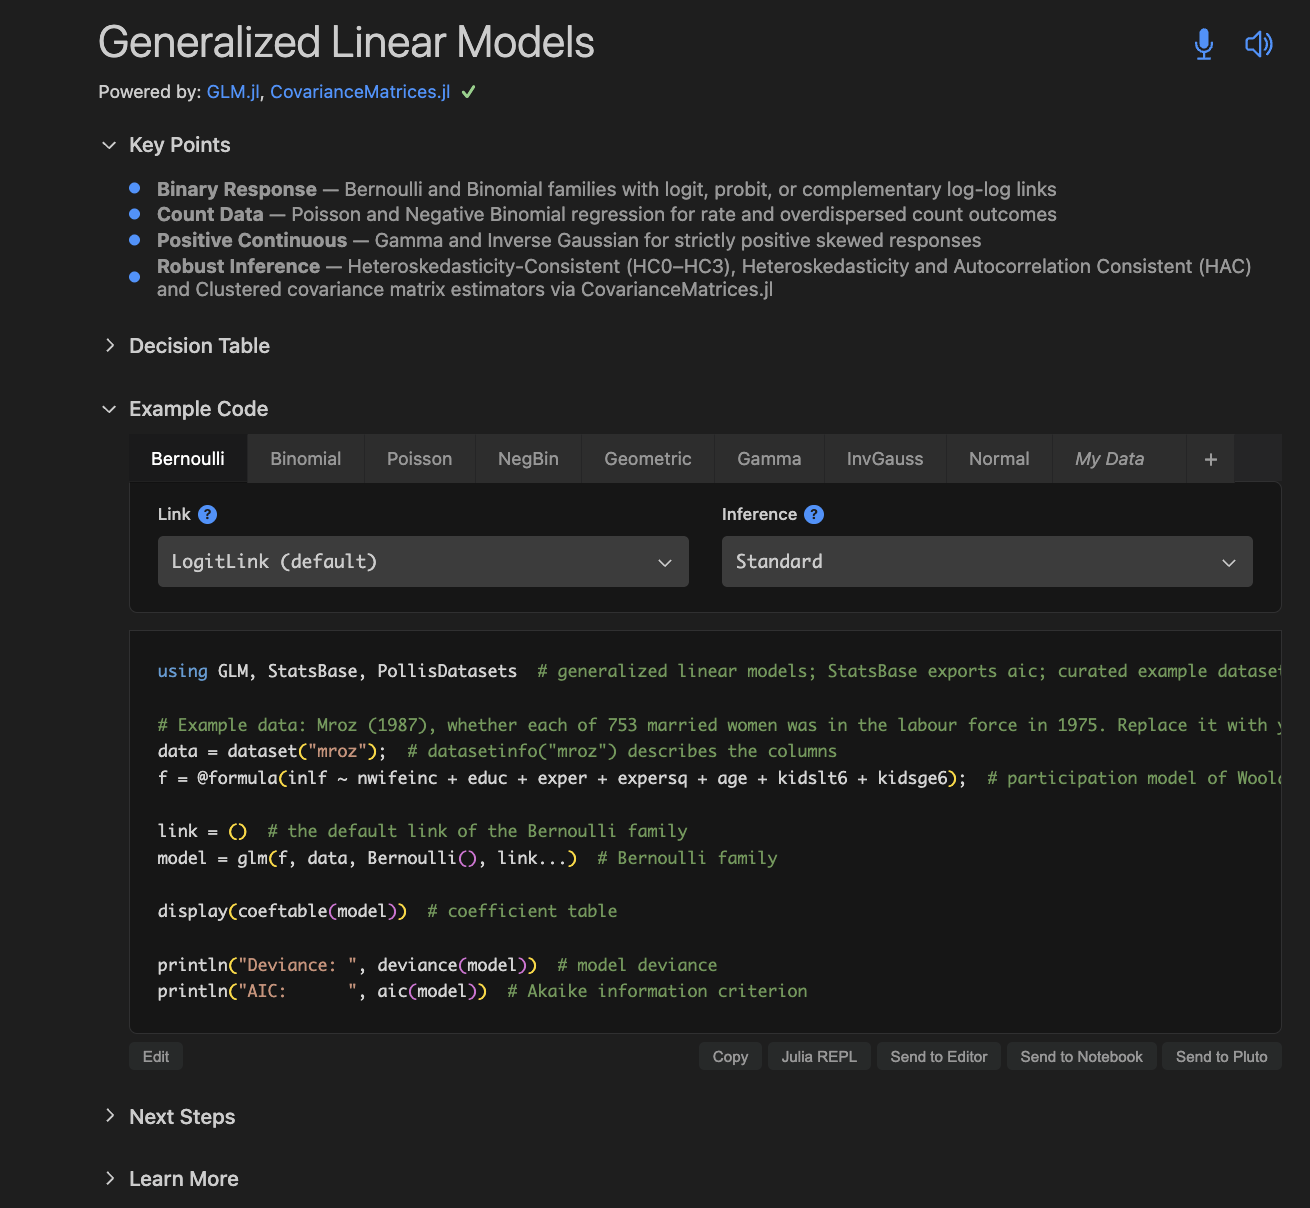
\includegraphics[width=0.62\linewidth]{glm.png}\end{center}

\subhead{From top to bottom}
\begin{itemize}
  \item \textbf{The title}, and the \ui{Powered by:} line: the Julia packages the panel uses, each a link to
    its documentation, with the tick or \ui{Install} (see Getting Started, page 2).
  \item \textbf{Key Points}: what the method does and when to use it, in a few lines.
  \item \textbf{Decision Table}, in some panels: which variant to use for which data.
  \item \textbf{Illustration}, in some panels: a picture of the method or its variants.
  \item \textbf{Example Code}: the tabs of the panel's variants (above, \ui{Bernoulli}, \ui{Binomial}, \ldots),
    its inputs, and the code. Changing an input changes the code at once.
  \item \textbf{Next Steps} and \textbf{Learn More}, at the bottom (next page).
\end{itemize}
Click a section's name to open or close it.

\subhead{Run the example}
The buttons below the code send it where you want it:
\begin{itemize}
  \item \ui{Julia REPL} runs it in the Julia REPL, starting it if needed.
  \item \ui{Send to Notebook} opens it in a new Jupyter notebook, with the Julia kernel.
  \item \ui{Send to Pluto} opens it in a new Pluto notebook, in Pollis's browser.
  \item \ui{Send to Editor} opens it in a new, unsaved Julia file, and \ui{Copy} copies it.
\end{itemize}
Code sent to the Julia REPL or to a notebook starts with the line that installs any missing package.

\newpage
\subhead{Make the example your own}
\begin{enumerate}[label=\arabic*.]
  \item Choose \ui{Edit} below the code, and change it: your data, your variables, your options.
  \item Choose \ui{Save}, or \ui{Cancel} to leave it as it was. A saved example is marked \ui{Customised},
    and the panel shows your version from then on.
  \item To go back to the original, choose \ui{Restore Default}, then \ui{Confirm Restore} within four
    seconds. Your version goes to the Trash.
\end{enumerate}

\subhead{Add a tab of your own}
\begin{enumerate}[label=\arabic*.]
  \item Choose \ui{+} at the end of the tabs, type a name and press \ui{Enter}.
  \item The new tab, marked \ui{Added}, opens empty, for editing: write or paste your code, and \ui{Save}.
  \item To remove it, choose the \ui{×} on the tab, then \ui{Delete}; it goes to the Trash.
\end{enumerate}
Your examples and tabs are files in \texttt{\textasciitilde/.pollis/examples}, one folder per panel. They are
kept when Pollis is updated.

\subhead{Next Steps}
Visualise, Diagnose, Predict, Compare, Interpret: examples that carry on from the Example Code, using its
results. Next Steps opens once you have run or sent the Example Code of the tab (the \ui{?} beside it says so).
Its examples have the same buttons, and can be edited and restored in the same way.

\subhead{Learn More}
\begin{itemize}
  \item \ui{Local Wikis}: a reference page on the method, in Pollis.
  \item \ui{Notebook Tutorials}: notebooks that work through the method.
  \item \ui{Multimedia Tutorials}: videos and talks. \ui{Add / Edit Video} adds your own.
  \item \ui{Explore References}: the papers and books behind the method, with \ui{Open in Browser} and
    \ui{Copy BibTeX to Clipboard}. \ui{Add / Edit Reference} adds your own, from BibTeX, a link or a DOI;
    they go into your references, in PollisReferences (page 40), and \ui{Edit} corrects a work wherever it is cited.
\end{itemize}

\begin{caution}{The example data are an example}
They show how the method works. To use it on your own data, change the lines that load the data,
and check that the variables and options still suit your question.
\end{caution}

\begin{trouble}
\textbf{Next Steps is dimmed} & Run or send the Example Code of this tab first. \\
\textbf{An error that a package is not found} & Use \ui{Julia REPL} or \ui{Send to Notebook}, which install it, or \ui{Install} on the \ui{Powered by:} line. \\
\textbf{The send buttons are greyed out} & Finish editing (\ui{Save} or \ui{Cancel}); an added tab needs some code first. \\
\end{trouble}

\begin{note}{Not available yet}
The microphone and speaker buttons beside the title: voice comes in a later version.
\end{note}

\seealso{Getting Started, page 2.\quad Data and Databases, page 6.\quad Customisation, page 8.}

% =====================================================================
% PAGES 6–7 — DATA AND DATABASES
% =====================================================================
\topic{Data and Databases}{Databases view · Explore > Access Files and Databases}{The datasets that come with Pollis, your own databases, and the Databases view.}

Pollis comes with a collection of real datasets, PollisDatasets, that its examples use, and connects to
DuckDB, SQLite and PostgreSQL databases. All the work with data is done in Julia: the Databases view shows
what is there and writes the code to reach it.

\subhead{PollisDatasets}
57 real datasets, such as \texttt{mroz}, \texttt{airpassengers}, \texttt{iris},
and \texttt{challenger}, each with its source and licence. In Julia:
\begin{itemize}
  \item \texttt{datasets()} lists them;
  \item \texttt{datasetinfo("mroz")} describes one and its columns;
  \item \texttt{data = dataset("mroz")} loads one as a Tables.jl table.
\end{itemize}
They are installed the first time the Julia REPL starts (Getting Started, page 2). When new datasets are
added, a notification says so.

\subhead{The built-in database}
The same datasets are also a DuckDB database, \emph{PollisDatasets}, one table per dataset, named after it,
with a description of the table and of each column. It is read-only, and is rebuilt only when
PollisDatasets changes. The Welcome page's \ui{Status} says when it is ready. Like the other built-in databases (page 40), it is a
DuckDB file, not in the Lance format: Pollis also brings DuckDB's Lance extension, for Lance datasets such
as tables of embeddings, but the built-in databases do not need it.
\begin{enumerate}[label=\arabic*.]
  \item Open the \ui{Databases} view, in the secondary side bar on the right (or choose
    \ui{Open Databases View} in the notification of new datasets).
  \item Click \ui{PollisDatasets}, marked \ui{built-in}. It connects in the Julia REPL as \texttt{pollis}.
  \item Expand it to see its tables and their columns.
\end{enumerate}
Then query it in the Julia REPL with SQL:
\begin{center}\texttt{DBInterface.execute(pollis, "SELECT * FROM mroz WHERE educ > 12")}\end{center}

\subhead{The Databases view}
\begin{itemize}
  \item Click a connection to connect it in the Julia REPL; \ui{Disconnect} closes it.
  \item On a table, \ui{Open in Table Viewer} shows its rows; right-click it for
    \ui{Preview Rows in Julia REPL}.
  \item \ui{Show Tables} and \ui{Hide Tables}, beside a connection, expand or collapse it;
    \ui{Refresh Schemas}, at the top of the view, shows tables you have just created.
  \item Right-click a connection for \ui{Copy Name}, \ui{Copy Connection Code}, \ui{Edit Connection} and
    \ui{Delete Connection}, which removes only the saved connection, never the database.
\end{itemize}

\subhead{Three ways to use SQL}
SQL should be at hand wherever you are working, without a second database program: all three use the
same DuckDB engine, with the Lance extension, and attach the four built-in databases, read-only.
\begin{itemize}
  \item \textbf{The \texttt{duckdb>} terminal}, for SQL alone, without starting Julia: \ui{New DuckDB
    Terminal}, at the top of the Databases view (or \ui{Databases: New DuckDB Terminal} in the Command
    Palette). It opens an empty database in memory; \texttt{.help} lists its commands, such as
    \texttt{.tables}, and Ctrl+C stops a long query.
  \item \textbf{The \texttt{sql>} mode} of the Julia REPL, for a query in the middle of Julia work: type
    \texttt{>} on an empty line, then the query, ending in \texttt{;}. The result is a Tables.jl table in
    \texttt{ans}, ready for Julia; Backspace on an empty line goes back to \texttt{julia>}.
  \item \textbf{\texttt{db = PollisDB.connect()}}, for Julia code and scripts: a DuckDB connection in
    memory, shown in the Databases view; \texttt{PollisDB.connect("sales.duckdb")} opens a file instead.
    Lance is loaded in the background, so the connection is ready at once.
\end{itemize}

\newpage
\subhead{Connect to your own database}
\begin{enumerate}[label=\arabic*.]
  \item In the Databases view, choose \ui{New}, then \ui{DuckDB}, \ui{PostgreSQL} or \ui{SQLite}.
  \item Give a \ui{Connection Name} and the \ui{Julia Variable} that will hold the connection, and choose
    whether to keep it for all your work (\ui{Global}) or for this folder only (\ui{Current Workspace}).
  \item For DuckDB or SQLite, choose the database file (\ui{Choose File}). A DuckDB connection with no file
    is an empty database in memory: it can read CSV and Parquet files in place, and is lost when you
    disconnect. \ui{Read Only} protects a file from changes.
  \item For PostgreSQL, give the \ui{Host}, \ui{Port}, \ui{Database} and \ui{Username}.
  \item Check the \ui{Generated Code}, then \ui{Save Connection}, or \ui{Connect} to save it and connect.
\end{enumerate}
A connection opened by your own code can be shown in the view as well:
\begin{center}\texttt{con = PollisDB.show(DBInterface.connect(DuckDB.DB, "sales.duckdb"); name = "Sales")}\end{center}

\begin{caution}{PostgreSQL passwords}
With \ui{Ask for Password in the REPL} (the default), you type the password in the Julia REPL when you
connect: it is never written in the code, in the REPL history or in a file. Without it, the password comes
from \texttt{PGPASSWORD} or \texttt{\textasciitilde/.pgpass}.
\end{caution}

\subhead{Panels for data}
\begin{itemize}
  \item \ui{Explore > Access Files and Databases}: \ui{SQL Databases} (query, import a CSV, Parquet or JSON
    file, save a table, export a query), \ui{CSV Files} and \ui{Excel Workbooks}.
  \item \ui{Explore > Access Data Libraries}: Hugging Face and Kaggle datasets, Yahoo Finance, Alpha Vantage,
    US SEC EDGAR, FRED and the European Central Bank. A provider that needs an API key shows
    \ui{Set API key} on the \ui{Powered by:} line; the key is kept in your system's secure storage.
\end{itemize}

\begin{trouble}
\textbf{The view shows no tables} & Choose \ui{Refresh Schemas}. A new database stays empty until you create a table in the Julia REPL. \\
\textbf{\ui{PollisDatasets} does not connect} & The Julia REPL has not started yet, or is still installing: wait for the Welcome page to say the database is ready. \\
\textbf{Cannot write to \texttt{pollis}} & The built-in database is read-only: save your tables in a database of your own. \\
\textbf{PostgreSQL does not connect} & Check the host, port and \ui{SSL Mode}; the \ui{Connection Timeout} is 10 seconds. \\
\end{trouble}

\begin{note}{Not available yet}
International Monetary Fund Datasets, World Bank Indicators and the Kenneth French Data Library are in
\ui{Access Data Libraries}, greyed out.
\end{note}

\seealso{Getting Started, page 2.\quad Collaboration, page 32, for sharing datasets and databases.}

% =====================================================================
% PAGES 8–9 — CUSTOMISATION
% =====================================================================
\topic{Customisation}{Pollis Views · Settings}{Showing only the menus you need, and making Pollis yours.}

Pollis has hundreds of panels. A \emph{View} is a named set of the menu items Pollis shows: a course can
keep only its own topics, a researcher only their field. The panels you hide are still there; another
View shows them again.

\subhead{Choose a View}
The name of the View in use is in the title bar, before the layout buttons: \ui{View: Max}. Click it for the
Views menu, with a tick on the one in use. Two Views are built in:
\begin{itemize}
  \item \ui{Max} shows every menu item. It is the default.
  \item \ui{Min} shows a short selection: the common plots and Descriptive Statistics in \ui{Explore},
    and a few models, simulations and optimisation panels.
\end{itemize}
Switching applies at once, to every menu. The built-in Views cannot be changed or deleted.

\subhead{Make a View of your own}
\begin{enumerate}[label=\arabic*.]
  \item In the Views menu, choose \ui{Create View...}, type its name, and choose the View it starts from:
    \ui{Max} starts with every menu item. Or choose \ui{Save View As...} to copy the View in use.
  \item The new View becomes the one in use, and the \ui{Views} panel opens in the secondary side bar,
    on the right, after \ui{Databases}: the menus, with every item below them.
  \item Untick an item to hide it, tick it to show it. Unticking a submenu hides everything in it; a
    submenu shows how many of its items are shown, such as \ui{4/12}. Changes apply at once.
\end{enumerate}
\ui{Explore}, \ui{Model}, \ui{Simulate}, \ui{Optimise}, \ui{Extend} and \ui{Compose} can be trimmed to the
items you tick; in the other menus, such as \ui{File} or \ui{Help}, you can hide single items.

\newpage
\subhead{Edit, delete and share Views}
\begin{itemize}
  \item \ui{Edit View...} makes one of your Views the one in use, and shows its items in the \ui{Views} panel.
  \item \ui{Delete View...} moves its file to the Trash, so it can be restored. Deleting the View in use
    switches to \ui{Max}.
  \item \ui{Open Views Folder} opens \texttt{\textasciitilde/.pollis/views}: each of your Views is a JSON file
    there. Copy a file to another computer, or give it to your students, to use the same View.
\end{itemize}
The View in use is kept in the setting \setting{pollis.view}.

\subhead{Settings}
Choose the \ui{Manage} gear at the bottom left, then \ui{Settings}, and type in the search box a word or a
setting's id, such as \setting{julia.startREPLOnStartup}. \ui{Themes > Color Theme}, in the same gear,
changes the colours, light or dark.

\subhead{Extensions}
The Extensions pane, in the activity bar on the left, installs extensions from Open VSX, the open
registry of extensions, as well as Pollis toolboxes (next topic). Some extensions published only by
Microsoft are not on Open VSX, so they cannot be installed in Pollis.

\subhead{What Pollis keeps for you}
Your own things are files in \texttt{\textasciitilde/.pollis}, kept when Pollis is updated:
\begin{center}\small
\begin{tabular}{@{}ll@{}}
\texttt{views} & your Views\\
\texttt{examples} & your Example Code and added tabs (Inside a Panel, page 4)\\
\texttt{workflows} & your copies of the replications (page 14)\\
\texttt{methods}, \texttt{packages} & your new methods and their packages (page 16)\\
\texttt{practice} & the exercises you write (the Learning and Practice toolbox)\\
\texttt{rss} & the items of your RSS feeds (page 22)\\
\end{tabular}
\end{center}

\begin{caution}{A hidden item is only hidden}
A View changes the menus, nothing else: the Command Palette and links between panels still reach every
panel. A View is not a way to stop students from opening a panel.
\end{caution}

\begin{trouble}
\textbf{A menu item has gone} & The View in use hides it: switch to \ui{Max}, or tick it in your View. \\
\textbf{The items cannot be ticked} & The View in use is built in: choose \ui{Save View As...} to make an editable copy. \\
\textbf{An extension is not found} & It is not on Open VSX. Look for an open alternative there. \\
\end{trouble}

\seealso{Toolboxes, page 10.\quad Inside a Panel, page 4.}

% =====================================================================
% PAGES 10–11 — TOOLBOXES
% =====================================================================
\topic{Toolboxes}{Extensions pane > Toolboxes · Compose > New Panels and Toolboxes}{Adding a whole field to Pollis with a toolbox extension.}

A toolbox is an extension that adds a set of panels to the menus, with their wikis and notebook
tutorials. It holds no program code: its panels are made like Pollis's own. Four are published:
\begin{itemize}
  \item \textbf{Financial Econometrics}: ARIMAX, VAR and VECM, GARCH-type and regime switching models,
    forecasting, Bayesian asset-pricing factor models.
  \item \textbf{Economics}: business cycle filters, stochastic volatility, DSGE and heterogeneous-agent
    models, continuous-time macro-finance, game theory.
  \item \textbf{Mathematical Core}: symbolic maths, linear algebra, nonlinear systems, numerical
    differentiation and integration, ordinary and partial differential equations.
  \item \textbf{Learning and Practice}: multiple-choice exercises whose data and answers Julia computes, and
    a panel to write new ones; described in its own guide, \emph{Learning and Practice}.
\end{itemize}

\subhead{Install a toolbox}
\begin{enumerate}[label=\arabic*.]
  \item Open the Extensions pane, in the activity bar on the left. The \ui{Toolboxes} section, at the top,
    lists the toolboxes you have not installed. Click a name for its details.
  \item Choose \ui{Install}. When Pollis asks, choose \ui{Reload Now} or \ui{Restart Extensions}.
  \item The \ui{Toolbox Panels} page opens: installing a toolbox does not change your menus until you
    choose its panels there (next page).
\end{enumerate}
An installed toolbox moves to the \ui{Installed} section. When a newer version is published, it comes back
to \ui{Toolboxes} with \ui{Update}.

\subhead{Choose its panels, and where they go}
The \ui{Toolbox Panels} page shows the toolbox on the left and \ui{Your Menus (Preview)} on the right.
\begin{enumerate}[label=\arabic*.]
  \item Tick the panels you want (\ui{Select All}, \ui{Select None}), or choose
    \ui{Display Author's Suggestion} to see where the author would put them.
  \item Click a blue line in the preview, \ui{Put here}, to put the ticked items there. A ticked toolbox
    menu moves with its panels inside; untick it to move panels out of it.
  \item Choose \ui{Publish}. The page then says \ui{In your menus as shown.}
\end{enumerate}
A toolbox can go in \ui{Explore}, \ui{Model}, \ui{Simulate}, \ui{Optimise} or their submenus, or in
\ui{Extend}, a menu that appears only when a toolbox puts something in it.

\newpage
To change them later, choose \ui{Edit} on the toolbox in the \ui{Installed} section, or \ui{Toolbox
Panels...} in the Command Palette (\ui{Compose: Toolbox Panels...}). To remove a toolbox, choose \ui{Uninstall} on it in the same section.

\subhead{Make a toolbox}
A teacher can package the panels of a course as one toolbox and give it to the students. This is done by
your coding agent (Orchestration, page 34), with a skill that writes the toolbox for you.
\begin{enumerate}[label=\arabic*.]
  \item Choose \ui{Compose > New Panels and Toolboxes > Package a Toolbox...} The agent starts in a terminal.
  \item Tell it which panels you want, by their menu titles, the menus they go in and their order, and the
    toolbox's name and description. It asks for what is missing.
  \item It writes a short spec, builds the toolbox and its README, and says where the \texttt{.vsix} file is.
  \item To install it, run \ui{Extensions: Install from VSIX...} in the Command Palette and choose the file.
    Your students do the same with the file you give them. Then choose its panels, as on the previous page.
\end{enumerate}
To change it, edit the spec, raise its version, build again and install the new file over the old one.

\subhead{New panels}
\ui{Compose > New Panels and Toolboxes > Create a Panel...} has your coding agent write a new panel with
you. \ui{Create Panels from a Request...} writes several at once from a request file, which lists the
toolbox and, for each panel, its topic, methods and menu. Without a request file open, it opens an
example to fill in. New panels can then be packaged as a toolbox.

\begin{caution}{Toolboxes need the Internet to install}
The list of toolboxes and their files come from GitHub. Once installed, a toolbox works offline.
\end{caution}

\begin{trouble}
\textbf{``Could not load the list of toolboxes''} & Check the Internet connection, then choose \ui{Retry}. \\
\textbf{Installed, but nothing in the menus} & Choose its panels and \ui{Publish}: \ui{Edit} on the toolbox, in \ui{Installed}. \\
\textbf{The \ui{Toolbox Panels} page is empty} & Reload the window or restart the extensions, as Pollis asked, first. \\
\textbf{A panel cannot go in a toolbox} & Some Pollis panels have code of their own and are marked not portable; the agent says which. \\
\end{trouble}

\seealso{Customisation, page 8.\quad Orchestration, page 34.}

% =====================================================================
% PAGE 13 — REPLICATION, METHODS AND WORKFLOWS (OVERVIEW)
% =====================================================================
\overview{Replication, Methods and Workflows}{Replay a classic. Keep what it teaches.}{Besides its replication record, a replicated article can leave two things behind: a new method, and a workflow.}

\begin{minipage}[t]{0.31\linewidth}\vspace{0pt}
\subhead{1\quad Replication}
It starts from an article, its input data, and either the results it publishes or its authors' code,
in any language. If a method the article uses is missing from Julia's packages, it is written first.
Then each result is printed beside the published one. Replication, page 14.
\end{minipage}\hfill
\begin{minipage}[t]{0.31\linewidth}\vspace{0pt}
\subhead{2\quad Methods}
A method an article needed and no Julia package had becomes a documented Julia package. Its tests run
the article's data and check the published results, within tolerances. It comes with a vignette, and can
be published in the Pollis registry. Methods, page 16.
\end{minipage}\hfill
\begin{minipage}[t]{0.31\linewidth}\vspace{0pt}
\subhead{3\quad Workflows}
A flat set of procedures, each with its inputs, its outputs and what it runs. Extracted from a
replication, it runs on your own data; combined with others, its independent procedures run side by side.
\end{minipage}

\vspace{6pt}
\begin{note}{Not available yet}
Replication records (the article, its data, the targets, the Julia code, whether the replication is full
or partial, and any differences); \ui{Compose > Replication > Replicate a Classical Article...}; and
\ui{Browse Workflows...}, \ui{Extract a Workflow...} and \ui{Combine Workflows...} in \ui{Compose > Workflows}.
\end{note}

\vfill
\begin{center}
  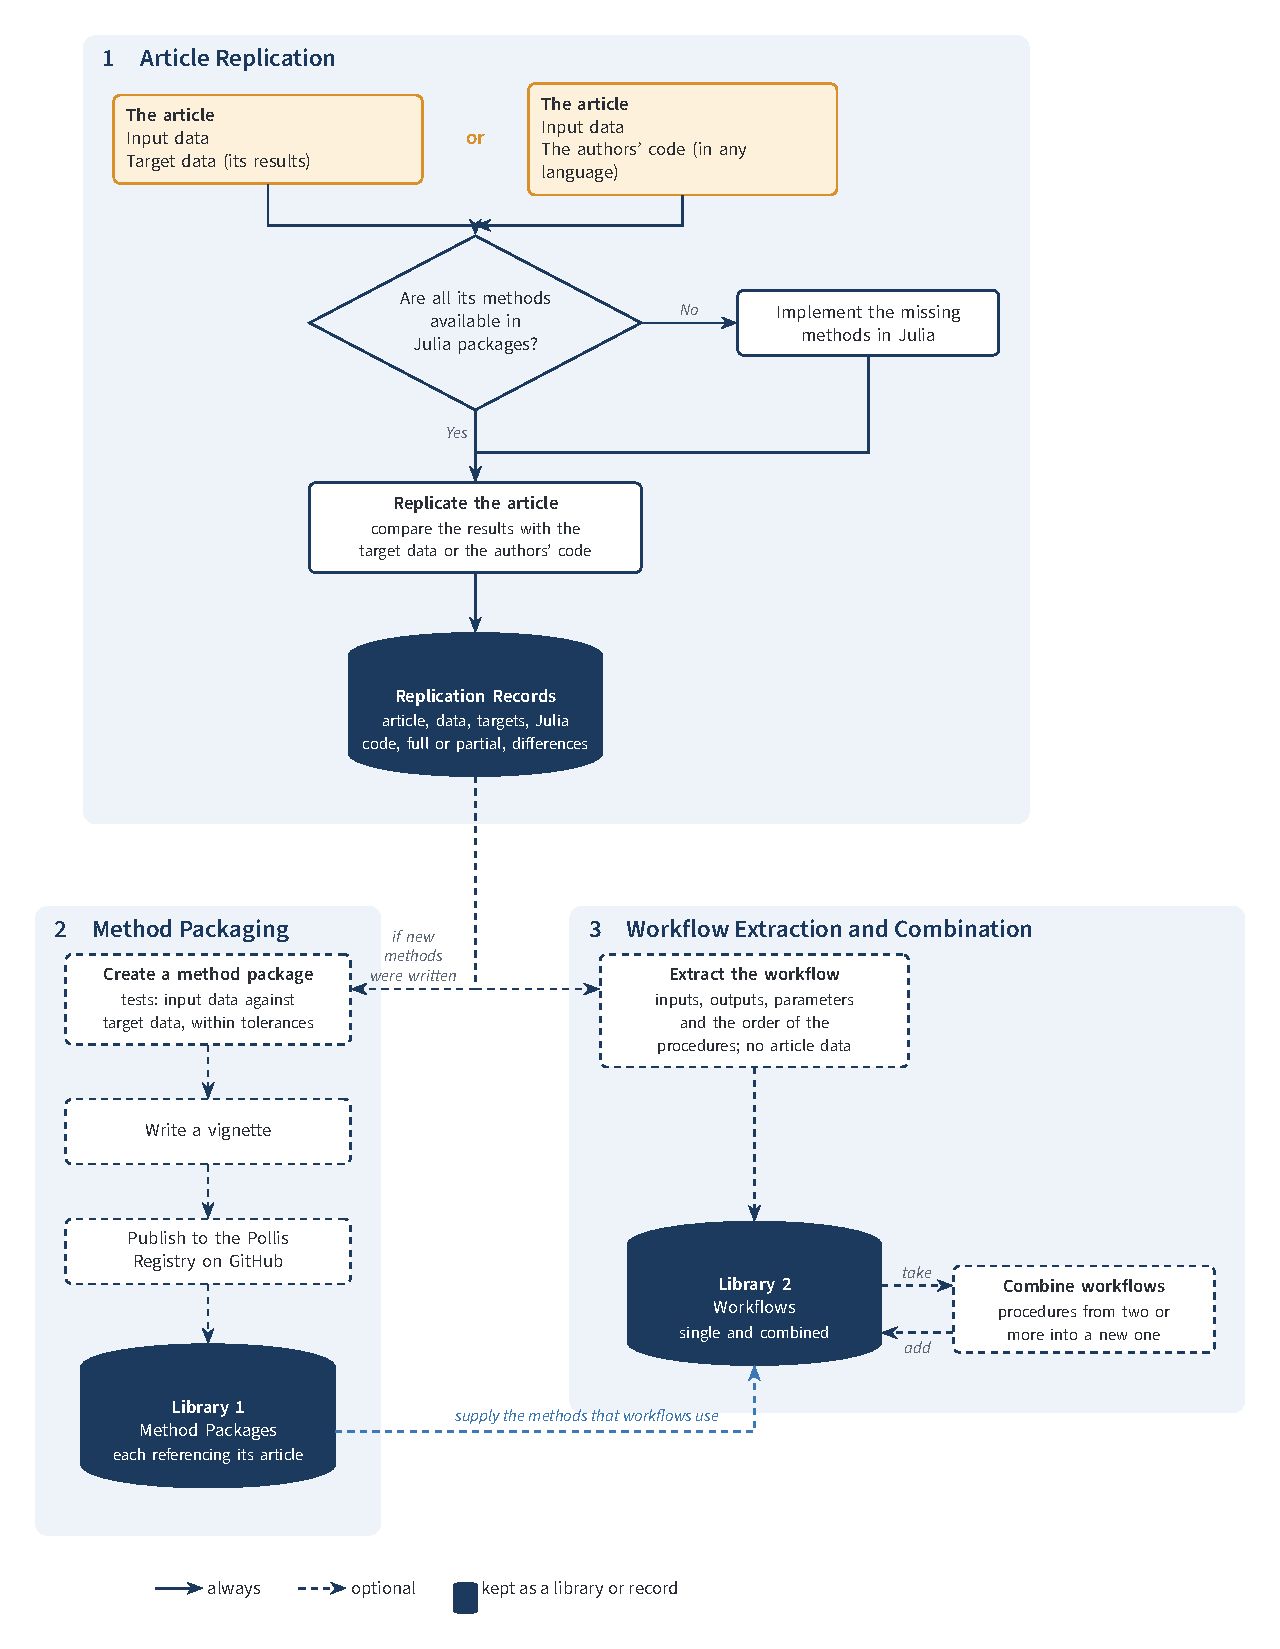
\includegraphics[height=0.62\textheight]{../workflows/replication_flowchart.pdf}
\end{center}
\vfill

% =====================================================================
% PAGES 14–15 — REPLICATION
% =====================================================================
\topic{Replication}{Compose > Replication}{Replaying a classic paper from its own data, step by step.}

A \emph{replication} reproduces a published analysis on its own public data: a Jupyter notebook
that follows the article section by section and prints every published value beside Julia's. It shows a
method at work on a real question, and that Julia gets the published answer.

\subhead{The replications}
\begin{center}\small
\renewcommand{\arraystretch}{1.15}
\begin{tabular}{@{}p{0.43\linewidth}p{0.53\linewidth}@{}}
\textbf{Replication} & \textbf{Article}\\
Panel data: is public capital productive? & Munnell (1990)\\
GARCH: volatility after non-trading days & Bollerslev and Ghysels (1996)\\
Survival: the Mayo model for primary biliary cirrhosis & Dickson et al.\ (1989)\\
Logistic regression: the Challenger O-rings & Dalal, Fowlkes and Hoadley (1989)\\
Threshold autoregression: the lynx and the sunspot cycles & Tong and Lim (1980)\\
Dynamic time warping: the UCR archive baselines & Dau et al.\ (2019)\\
Propensity score matching: the NSW experiment and its replications & Dehejia and Wahba (1999)\\
Random forests: Breiman (2001) & Breiman (2001)\\
LSTNet: long- and short-term patterns in multivariate time series & Lai, Chang, Yang and Liu (2018)\\
\end{tabular}
\end{center}

\subhead{Open a replication}
\begin{enumerate}[label=\arabic*.]
  \item Choose \ui{Compose > Replication > Browse Replications...}
  \item The page lists the replications with their article (its DOI, or \ui{Web Page} when it has none, and \ui{Copy BibTeX}), the
    Julia packages and datasets they use, their size, any data they download, and the date they were last
    updated. Click \ui{more} under a description to read it all.
  \item Click a replication's name. The first time, Pollis makes your own copy in
    \texttt{\textasciitilde/.pollis/workflows}, and opens its notebook.
\end{enumerate}
Your copy is yours to change: later openings show it as you left it.

\newpage
\subhead{Follow it}
\begin{enumerate}[label=\arabic*.]
  \item Choose the Julia kernel if the notebook asks for one.
  \item Run the cells in order, from the top. The first code cell, \texttt{Pollis.packages(...)}, installs
    any package that is missing, so the first run takes longer.
  \item Read each section beside the article: the text says which table, figure or page it
    replicates.
\end{enumerate}
The data come from PollisDatasets or from the source the article used. The page says when a
replication downloads data, and how much (\ui{+ \emph{size} download}); \ui{download if asked} marks data
that it downloads only when you agree.

\subhead{Checking the results}
Most comparisons are small tables: Julia's value in full, the same value rounded as the article prints it,
the published value, and the number of decimals they share, or \texttt{DIFFERENT}. Each table's title
says where the published value is printed, usually a page or table. Random forests averages 100 random runs, as Breiman did, so it
asks instead whether Julia's average and Breiman's differ by less than two standard errors. All the
notebooks but the panel-data one end with a section, \emph{What differs, and why}.

\subhead{New and updated replications}
New replications, and new versions of the ones you have, can arrive between releases of Pollis: the page
marks them \ui{New} or \ui{Updated} until you open them. When your copy is older than the new version, the
page says \emph{Your copy is older than this version} and offers \ui{Open Updated Version}: the new notebook
is saved beside yours, with its date in the name, and your copy is kept.

\begin{note}{From a replication to a report}
A replication's notebook can become a LaTeX report or slides: Reports, page 20. The GARCH replication has
its own report template.
\end{note}

\begin{trouble}
\textbf{A cell fails: a package is not found} & Run the first code cell, \texttt{Pollis.packages(...)}, then the others in order. \\
\textbf{A download fails} & Check the Internet connection; the source may be down for a while. Try again later. \\
\textbf{You changed your copy and want the original} & Rename or delete its folder in \texttt{\textasciitilde/.pollis/workflows}; opening the replication again makes a fresh copy. \\
\end{trouble}

\begin{note}{Not available yet}
\ui{Replicate a Classical Article...} is in the menu but not built yet: it says so when chosen. So are
\ui{Browse Workflows...}, \ui{Extract a Workflow...}, \ui{Combine Workflows...}, \ui{Create Operational Workflow...} and
\ui{Automations...}, in \ui{Compose > Workflows}.
\end{note}

\seealso{Reports, page 20.\quad Methods, page 16.\quad Data and Databases, page 6.}

% =====================================================================
% PAGES 16–17 — METHODS
% =====================================================================
\topic{Methods}{Compose > Methods}{Turning a new method into a tested Julia package, with its vignette.}

A \emph{new method} is one no Julia package has yet, taken from an article: its data, the results the
article publishes for them, and the code that reproduces them. Pollis makes it a Julia package whose tests
are the published values, with a \emph{vignette}, its documentation, and can publish it in the Pollis
registry. Without data and expected results there is no new method.

\subhead{Start a method}
Choose \ui{Compose > Under Construction...}. The method's page has five numbered steps, below;
its title is at the top: click it to change it. Nothing is saved until you type or add something.
Each method is a folder in \texttt{\textasciitilde/.pollis/methods}.

\subhead{1. Article and Data}
\begin{itemize}
  \item \ui{Article}: the \ui{Article Link}. Pollis opens it in the integrated browser and keeps no copy;
    \ui{Save a Copy...} saves one outside Pollis, by default in the \texttt{data} folder of your Pollis
    Workspace (Reports, page 20).
  \item \ui{Input Tables}, the data the method is computed from: \ui{Empty Table} to type one in,
    \ui{Add from a Link}, \ui{Add from PollisDatasets}, or \ui{Add from Article}: give the numbers of the
    article's tables, such as \texttt{3.2, 5.8}, and click \ui{Ask Agent}.
  \item \ui{Target Tables}, the published results the method must reproduce: \ui{Empty Table},
    \ui{Add from CSV Files}, or \ui{Add from Article}. Every printed value becomes a test of the package.
\end{itemize}
A table typed in by the agent keeps every value as printed, and the agent lists the values it could not
read for certain: check them against the article. The tests are only as right as the targets.

\newpage
\subhead{2. Write a Method}
Write \ui{Instructions} for the agent, saved in \texttt{INSTRUCTIONS.md}: what the method does, where it is
in the article, what to watch for. Then click \ui{Write Method}: your coding agent writes the code in
\texttt{src}, with you, and runs the tests. \ui{Edit method.toml} shows the method's own file: its tables,
its call and its article. \ui{Open Code} opens the code.

\subhead{3. Write a Vignette}
Once the method's tests pass, write notes on the vignette (\texttt{VIGNETTE.md}) and click \ui{Write
Vignette}: the agent writes it in LaTeX, with its PDF. \ui{Edit Vignette} and \ui{Open PDF} open them.

\subhead{4. Prepare for Registration}
Give the \ui{Package Name}: a capital letter, then letters and digits, such as \texttt{ThresholdAR}; the
Pollis registry asks for at least 5 characters. It also asks for a usage example and a docstring for every
exported name: \ui{Prepare for Registration} has the agent check the method and fix what it can.

\subhead{5. Package and Publish}
Each button runs in a terminal. \ui{Package and Test} makes the package in
\texttt{\textasciitilde/.pollis/packages}, runs its tests and checks the registry rules. \ui{Package, Test
and Push to GitHub} then pushes it to its own public repository, if its tests all pass. \ui{Package, Test,
Push and Register} then registers it, if it meets the rules. Pushing needs a \ui{GitHub Owner}, a user or
organization, and the GitHub CLI, \texttt{gh}, signed in; Pollis asks first: \emph{Push to GitHub as
\ldots?}

\subhead{Browse methods and read vignettes}
\ui{Compose > Methods > Browse Methods} lists yours, \ui{In Progress} and \ui{Published by You},
then the \ui{Library} of nine methods by Pollis, from arc-fs to threshold autoregression: click one to open
your own copy. \ui{Delete} and \ui{Delete Empty Methods} move folders to the Trash. \ui{Help >
Documentation > Package Vignettes} lists the vignettes of installed packages (they open offline) and, with the
Internet, those \ui{In the Registry}.

\begin{caution}{The agent steps cost tokens}
Add from Article, Write Method, Write Vignette and Prepare for Registration run your coding agent, on your
account.
\end{caution}

\begin{trouble}
\textbf{\emph{\ldots has no target tables, so nothing to test}} & Add the published results in \ui{Target Tables}. \\
\textbf{\emph{Copies are kept outside Pollis}} & Save the copy outside \texttt{\textasciitilde/.pollis}, e.g.\ in a Pollis Workspace. \\
\textbf{The push fails} & Sign in with \texttt{gh auth login} in a terminal, and check the GitHub Owner. \\
\end{trouble}

\seealso{Replication, page 14.\quad Orchestration, page 34.}

% =====================================================================
% PAGES 18–19 — POLLIS PACKAGES
% =====================================================================
\topic{Pollis Packages}{github.com/Trumpingtons}{The Julia packages written for Pollis, which you can also use without it.}

Most panels use Julia packages from Julia's General registry. Fourteen packages are Pollis's own: nine
methods, and five packages behind panels and features. All are public on GitHub, under
\href{https://github.com/Trumpingtons}{Trumpingtons}, with the MIT licence, and work in any Julia session,
with or without Pollis. None is in the General registry.

\subhead{The method packages}
The nine methods of the \ui{Library} in \ui{Compose > Methods > Browse Methods} (Methods, page 16).
Each is tested against the published results of the article it comes from, has a vignette, and is in the
Pollis registry.

\smallskip
{\small\renewcommand{\arraystretch}{1.25}%
\begin{tabularx}{\linewidth}{@{}>{\bfseries}l>{\raggedright\arraybackslash}p{0.27\linewidth}>{\raggedright\arraybackslash}X@{}}
\textcolor{navy}{\bfseries Package} & \textcolor{navy}{\bfseries Topic} & \textcolor{navy}{\bfseries Tested against} \\
ArcFS & Boosting & Breiman's arc-fs, from his random forests article \\
BreslowCox & Survival analysis & The Mayo model of primary biliary cirrhosis \\
ErrorComponents & Panel econometrics & Baltagi's tables for the Grunfeld, gasoline and public capital data \\
ForestOOB & Random forests & Breiman's out-of-bag errors and variable importance \\
GLMExtras & GLM inference & Dalal, Fowlkes and Hoadley's Challenger O-ring analysis \\
LSTNet & Time series forecasting & Lai, Chang, Yang and Liu's LSTNet-Skip and their PyTorch code \\
PeriodicGARCH & Volatility & Bollerslev and Ghysels's periodic GARCH \\
PropensityMatching & K-nearest neighbours & Dehejia and Wahba, and its replications \\
ThresholdAR & Nonlinear dynamics & Tong and Lim's threshold autoregression \\
\end{tabularx}}

\subhead{Install a method package}
Add the Pollis registry once, then add packages by name, in the Julia REPL's package mode (type \texttt{]}):

\smallskip
{\small\texttt{pkg> registry add https://github.com/Trumpingtons/PollisRegistry}\\
\texttt{pkg> add ThresholdAR}}

\smallskip
\ui{Help > Documentation > Package Vignettes} opens the vignettes of the packages you installed.

\newpage
\subhead{Packages behind panels and features}
{\small\renewcommand{\arraystretch}{1.25}%
\begin{tabularx}{\linewidth}{@{}>{\bfseries}l>{\raggedright\arraybackslash}p{0.36\linewidth}>{\raggedright\arraybackslash}X@{}}
\textcolor{navy}{\bfseries Package} & \textcolor{navy}{\bfseries What it does} & \textcolor{navy}{\bfseries Where Pollis uses it} \\
PollisDatasets & 57 small, well-known datasets for examples and teaching, as Tables.jl column tables &
  The built-in database (Data and Databases, page 6), \ui{Add from PollisDatasets} in Methods, and the
  examples of panels and replications \\
PollisTeX & Typesets LaTeX from Julia with Tectonic, downloaded on first use &
  \ui{Compose > Reports} (Reports, page 20) \\
EDGAR & Fetches SEC EDGAR filings and financial data &
  \ui{Explore > Access Data Libraries > US SEC EDGAR} \\
HARE & Heteroskedasticity and autocorrelation estimators &
  \ui{Model > Linear Models}: \ui{Linear Models with Heteroskedasticity}, \ui{with Autocorrelation} and
  \ui{with Heteroskedasticity + AR(1)} \\
RangeVol & Range-based volatility estimators &
  The Range-Based Volatility Estimation panel, not in the menus at present \\
\end{tabularx}}

\subhead{Install one}
Pollis installs these packages by itself when a panel, a replication or a report needs them. To install one
yourself, give its GitHub address, in the Julia REPL:

\smallskip
{\small\texttt{import Pkg; Pkg.add(url = "https://github.com/Trumpingtons/HARE.jl")}}

\begin{note}{The datasets' own terms}
The MIT licence covers PollisDatasets' code. Each dataset keeps the terms of its provider:
\texttt{datasetinfo("penguins")} shows its description, the source to cite, its licence and its columns.
\end{note}

\begin{trouble}
\textbf{\texttt{add ThresholdAR}: the package is not found} & Add the Pollis registry first, as above. \\
\textbf{\texttt{Pkg.add("HARE")}: the package is not found} & These five are in no registry: install with \texttt{Pkg.add(url = ...)}, as above. \\
\end{trouble}

\seealso{Methods, page 16.\quad Data and Databases, page 6.\quad Reports, page 20.}

% =====================================================================
% PAGES 20–21 — REPORTS
% =====================================================================
\topic{Reports}{Compose > Reports}{From a notebook to a LaTeX report or slides.}

Any Jupyter notebook, a replication's or your own, can become a LaTeX report (an article) or beamer slides,
with its outputs and figures and a PDF beside it. Pollis does this in its Julia REPL, without an agent;
a coding agent can then polish the draft into a finished document.

\subhead{Before you start: a Pollis Workspace}
Reports are written in the \texttt{reports} folder of a \emph{Pollis Workspace}: an ordinary folder for
your own work, outside Pollis. To make one, choose \ui{File > New Pollis Workspace...}, then choose or
create a folder, for example in your Documents, and click \ui{Make Pollis Workspace}. Pollis puts a
\texttt{pollis.toml} file and a \texttt{data} folder in it, and opens it. Next time, open that folder with
\ui{File > Open Folder...}.

\subhead{Make a report or slides}
\begin{enumerate}[label=\arabic*.]
  \item Open the notebook, for example your copy of a replication (page 14).
  \item Choose \ui{Compose > Reports > Export Notebook as LaTeX...} for a report, or \ui{Make Slides from
    a Notebook...} for slides. The notebook's own toolbar has the same two in its \ui{Export} button:
    \ui{LaTeX Report...} and \ui{Beamer Slides...}. With no notebook open, Pollis asks you to choose one,
    starting in \texttt{\textasciitilde/.pollis/workflows}.
  \item The Julia REPL installs PollisTeX if it is missing, runs the notebook's code cells in order and
    compiles the document.
  \item The \texttt{.tex} opens in the editor, and the PDF beside it, in the integrated browser.
\end{enumerate}
The files are in \texttt{reports/\emph{NAME}} of the workspace, \emph{NAME} being the notebook's:
\texttt{report.tex} or \texttt{slides.tex} and its PDF, each cell's printed output in
\texttt{outputs/cellN.txt}, and its figure in \texttt{figures/cellN.pdf}.

\newpage
\subhead{What the draft holds}
\begin{itemize}
  \item A \emph{report} is a draft of the notebook's text cells, with the printed outputs and figures in
    their place and without the code.
  \item \emph{Slides} have a frame for the text under each heading, and one for each output and each
    figure.
  \item A notebook with a \emph{template}, a \texttt{latex} folder beside it, gets that document instead,
    with its own tables, figures and references. The GARCH replication ships one for its report.
\end{itemize}

\subhead{Edit and compile}
Edit the \texttt{.tex} as you like, then click \ui{Compile LaTeX}, the play button at the top right of its
editor: Pollis saves it, compiles it with PollisTeX in the Julia REPL and reloads the PDF. Exporting the
notebook again refreshes the outputs and figures, and keeps your \texttt{.tex}: Pollis writes it only when
the folder has none. To start the draft again, delete the \texttt{.tex} first.

\subhead{Polish with Agent}
\begin{enumerate}[label=\arabic*.]
  \item Open the report's or the slides' \texttt{.tex}.
  \item Choose \ui{Compose > Reports > Polish with Agent...} The coding agent starts in a terminal in the
    report's folder.
  \item It turns the draft into a finished document: sections, tables, captions and citations, from the
    numbers already computed. It does not run the notebook again, and it compiles the document as it
    goes: the PDF beside you reloads each time.
\end{enumerate}
Polish runs on the Light tier of Model Routing (Orchestration, page 34).

\begin{caution}{Polish costs tokens}
The menu item with the sparkle runs your coding agent, on your account. Read the result: an agent can
still misplace a value, so check the numbers against the draft.
\end{caution}

\begin{trouble}
\textbf{\emph{Reports are written in the reports folder of a Pollis Workspace}} & Click \ui{New Pollis Workspace...}, or open your workspace folder. \\
\textbf{\emph{A Pollis Workspace keeps your work outside Pollis}} & Choose a folder outside \texttt{\textasciitilde/.pollis}, for example in your Documents. \\
\textbf{No PDF appears} & A cell or the compile failed: read the error in the Julia REPL, fix it, and export or compile again. \\
\textbf{Polish says to open the .tex} & Open \texttt{report.tex} or \texttt{slides.tex} first, then choose \ui{Polish with Agent...} again. \\
\end{trouble}

\seealso{Replication, page 14.\quad Orchestration, page 34.}

% =====================================================================
% PAGES 22–23 — RSS FEEDS
% =====================================================================
\topic{RSS Feeds}{Explore > RSS > RSS Feeds · Databases view > PollisRSS}{Following news, journals, central banks, searches, podcasts and videos, and keeping what they bring.}

\ui{Explore > RSS > RSS Feeds} opens a page with the feeds you follow on the left, by topic, and their
items on the right. Pollis reads every feed when it starts and then every hour; \ui{Refresh} reads them at
once. The feeds are read by your computer, not by a server of Pollis. At first, Pollis follows only the Julia news;
a notification at the first launch points to the catalogue, where you choose the rest.

Every feed is RSS to Pollis, wherever it comes from: most come from the \emph{catalogue}, about 520 feeds in 35 categories, from PollisRSS.jl and updated without a new Pollis,
ranging from Classics and Philosophy to Economics and Astronomy, all listed on the page in alphabetical order; some are
\emph{searches} you save, at arXiv or PubMed; and some are \emph{email alerts}, saved searches whose results
arrive by email, which Pollis turns into feeds. They are read, shown, archived and added to Zotero alike.

\subhead{Add a feed}
\ui{Explore > RSS > Add Feed...}, or \ui{Add Feed} on the RSS Feeds page, opens a page with these sections:
\begin{center}\small
\begin{tabular}{@{}lp{0.66\linewidth}@{}}
\ui{From an Address} & a feed's address, the page of a journal or a website, or a YouTube channel or its @handle; \ui{Find}\\
\ui{From a Search} & a PubMed or arXiv search, such as \texttt{abs:"survival analysis" AND cat:stat.ME}; \ui{Preview} first\\
\ui{From Email Alerts} & the alerts mailbox, and the alerts that arrived in it, ticked to follow (below)\\
\ui{Your Feeds} & the feeds you added, with \ui{Remove}; under \ui{Removed Feeds}, \ui{Restore}\\
\end{tabular}
\end{center}
For a journal's page at Wiley, Taylor \& Francis, SAGE, Elsevier, Cambridge Core or Oxford Academic, \ui{Find} gets the feed of
its newest issues; for another website, the feeds its page lists, to choose from when there are several.
Then pick the topic to list the feed under, or \ui{New Topic...}.

\subhead{Read}
\begin{enumerate}[label=\arabic*.]
  \item Click a topic or a feed on the left to see its items, or \ui{All Feeds}. The feeds of a topic are
    indented under it, with a camera after the name of a feed of videos and a microphone after a podcast's. Every topic of the catalogue is listed; one with no feed subscribed starts collapsed. The last column, \ui{Unread / Total}, counts the items of the \ui{Items From} period. The items are shown
    100 at a time, newest first; \ui{Previous} and \ui{Next}, above and under them, turn the pages.
  \item Click an item to open it in your browser; it is then marked read, and its title is no longer bold.
    \ui{Mark Unread}, shown when the pointer is on a read item, marks it unread again. An item of a podcast or a video has a \ui{Listen} or \ui{Watch} link; Pollis tells them
    by the feed, or by the item's address (a news site's video or audio page).
  \item Three columns of circles, for a feed or for all the feeds of a topic: green when on, red when off, half green and half red when only some of a topic's feeds are on; the last two are under \ui{Display}. \ui{Subscribed}: Pollis reads the
    feed every hour, and a catalogue feed ticked is followed (its count is a dash until then); unticked, it is no longer read, but its items stay. \ui{Here}: its items are shown on this
    page; unticked, they are hidden here and on the welcome page, but the feed is still read and archived, and
    the right says \ui{No items shown} when every item of a choice is hidden. \ui{Welcome Page}: its newest
    unread items are in the welcome page's \ui{RSS} section.
  \item \ui{Items From} sets how far back items are shown: \ui{The Last 7 Days}, \ui{30} (the default),
    \ui{90}, or \ui{All Items Kept}. Items without a date are always shown. \ui{On a Day...} shows the items of
    one day, chosen in a calendar. Only the latest items of each feed are kept here, and the archive goes back
    only to the day you started following it: a feed cannot tell what happened before then.
  \item An item of a journal has a purple tag: the journal's level in the Norwegian register (\ui{Level 2}
    leading, \ui{Level 1} academic, \ui{Level 0} not academic), OpenAlex's 2-year mean citedness
    (\ui{Cited 7.9}), and, once you have imported them (Built-in Databases, page 40), the SJR or Impact Factor
    quartile and its year (\ui{SJR Q1 2025}). The pointer on the tag shows every value known, with its source
    and year: SJR and its categories, SNIP, IPP, h-index, open access. Pollis knows the journal of a catalogue
    feed, of an email alert's article, and of a feed you added, by looking up its first items once.
  \item \ui{Journals}, next to \ui{Items From}, shows only the items of some journals: \ui{Academic (Level 1 or 2)},
    \ui{Leading (Level 2)}, \ui{Open Access}, and, once imported, \ui{SJR Q1}, \ui{SJR Q1--Q2} and \ui{SNIP Above 1}.
    Items not from a journal (news, blogs, preprints) always stay, and the counts follow the choice.
\end{enumerate}
\ui{Remove}, shown when the pointer is on a feed, takes it off the page; \ui{Restore}, under \ui{Removed Feeds} on the \ui{Add Feed} page, brings it back.

\subhead{Journal metrics}
\ui{Explore > RSS > Journal Metrics}, \ui{More Metrics...} in \ui{Journals}, the \ui{i} next to it, or a click on a tag
opens the \ui{Journal Metrics} page: each source's metrics, their values and meaning, and more to import (page 40).

\newpage
\subhead{Zotero}
\begin{itemize}
  \item \ui{Add to Zotero}, shown when the pointer is on an item, adds it to Zotero 7 or later, open on the
    same computer: an article from PubMed as a journal article, an arXiv, medRxiv or bioRxiv paper as a
    preprint, a video or a podcast episode as such, and anything else as a web page. When Zotero has
    collections, Pollis asks which one, starting from the last one you chose. The item then shows
    \ui{In Zotero}, and is listed in the \texttt{zotero} view of PollisRSS (below), with the collection.
  \item For an open-access paper, an arXiv, bioRxiv or medRxiv preprint or a PLOS article, Zotero also
    downloads its PDF and attaches it. For any other article, use Zotero's own \ui{Find Available PDF}
    (right-click the item in Zotero), which finds a free copy when there is one.
  \item \ui{Export as OPML} saves the feeds you follow as one file, to follow them in Zotero
    (\ui{File > New Feed > From OPML...}) or another feed reader. PubMed searches and email alerts are left
    out, since only Pollis reads them.
\end{itemize}

\subhead{The PollisRSS database}
Every item Pollis reads is added to a monthly file in \texttt{\textasciitilde/.pollis/rss/items}, so an item
stays when its feed drops it. \emph{PollisRSS} is a DuckDB database over those files, made with PollisDatasets the first time the Julia
REPL starts (Data and Databases, page 6), and empty until feeds are read:
\begin{enumerate}[label=\arabic*.]
  \item In the Databases view, click \ui{PollisRSS}, marked \ui{built-in}. It connects in the Julia REPL as
    \texttt{rss}, read-only.
  \item Query its four views: \texttt{items}, one row per item (feed, topic, title, link, published,
    received, summary, picture and media); \texttt{feeds}, one row per feed with its number of items;
    \texttt{zotero}, the items added to Zotero; and \texttt{episodes}, the podcast episodes downloaded.
\end{enumerate}
\begin{center}\small\texttt{DBInterface.execute(rss, "SELECT topic, count(*) FROM items GROUP BY topic")}\end{center}

\subhead{Podcasts}
An item of a podcast has \ui{Download Episode}, which saves its audio file in
\texttt{\textasciitilde/.pollis/rss/episodes}, a folder per podcast; the notification's \ui{Open Folder}
shows it, and the item then shows \ui{Downloaded}. The episode is listed in the \texttt{episodes} view of
PollisRSS, with the file. Videos are not downloaded, since YouTube's terms do not allow it, and news pages
stay links.

\subhead{Email alerts}
Google Scholar, JSTOR, HeinOnline, Nexis Uni, SSRN, Semantic Scholar, Web of Science, Scopus, Westlaw and
Factiva send the results of a saved search only by email. Send them to an address of your own, best one used
only for alerts, and Pollis turns each alert into a feed, with the title, the link, and the authors and journal
of each result. Pollis reads the mailbox on your computer over IMAP, read only: nothing passes through a server.
\begin{enumerate}[label=\arabic*.]
  \item \ui{Add Feed}, \ui{From Email Alerts}: the address, its IMAP server (suggested for Gmail, iCloud, Yahoo,
    Fastmail and GMX) and its password, kept in the system's keychain; then \ui{Connect}. Gmail, iCloud and Yahoo need an
    \emph{app password}; Outlook.com does not let programs in with a password.
  \item Create the alerts at each source, sent to that address. The \ui{Email Alerts} skill, in
    \ui{Compose > Agent Skills}, walks you through each source and writes precise searches in its syntax,
    so the alerts bring few false hits.
  \item \ui{Alerts in the Mailbox} lists the alerts that have arrived, by source; the ones you tick are
    listed under the topic \ui{Email Alerts}.
\end{enumerate}
Google Alerts (\ui{Show options > Deliver to > RSS feed}) and the table-of-contents alerts of many
publishers are feeds already: paste their address in \ui{From an Address}; \ui{Search Feeds from Other Services} there shows where EBSCOhost and ProQuest give theirs.

\begin{note}{Alerts on quotes, SEC filings and economic data}
Warnings when a quote crosses a level, a company files at the SEC or a series publishes a new value are not feeds: Alerts, page 26.
Press releases from PR Newswire, and what the news said around an event: Media Coverage, page 24.
\end{note}

\begin{trouble}
\textbf{\emph{Could not be read the last time; the items shown are the ones read before}} & The feed's site did not answer, or moved: try \ui{Refresh} later, or remove the feed and add its new address. \\
\textbf{\emph{No feed found at this address}} & On the journal's page, look for an RSS link and copy its address; for an Oxford journal, the RSS icon on its page. \\
\textbf{\emph{The mailbox could not be read}} & Check the address, the server and the password; Gmail, iCloud and Yahoo need an app password, and IMAP turned on. \\
\textbf{\emph{Zotero is not open}} & Open Zotero 7 or later on this computer, and click \ui{Add to Zotero} again. \\
\textbf{\emph{The episode could not be downloaded}} & The podcast's site did not answer: check the internet connection and click \ui{Download Episode} again. \\
\textbf{A YouTube channel shows no videos} & YouTube's feeds are sometimes unavailable for a while: the items come at a later reading. \\
\end{trouble}

\seealso{Data and Databases, page 6.\quad Alerts, page 26.}

% =====================================================================
% PAGES 24–25 — MEDIA COVERAGE
% =====================================================================
\topic{Media Coverage}{Explore > Media Coverage}{What the news said about a company, an institution or a subject, and when.}

\ui{Explore > Media Coverage} counts the articles about a company, an institution or a subject over a
period, by hour, day or week, marks the FOMC's releases, a company's SEC filings or a time of your own on
the same chart, and lists the articles, newest first. Pollis shows the headlines and links only; an article
opens in the internal browser.

\subhead{Search}
\begin{enumerate}[label=\arabic*.]
  \item \ui{Words}: what the articles must have. Quotes keep a phrase together (\texttt{"Apple Inc"}); \texttt{OR}
    between words takes any of them, in parentheses: \texttt{(iPhone OR iPad)}. Words can be a subject,
    such as \texttt{"going concern"}, or an institution: \texttt{"FOMC" OR "Federal Reserve"}.
  \item \ui{Sources}: tick the ones to search; Pollis keeps your choice. \ui{Yahoo Finance} has a
    \ui{Ticker} box beside it (\texttt{AAPL}): its headlines, and the company's SEC filings for \ui{Mark}.
  \item \ui{Period}: \ui{Last 24 Hours}, \ui{Last 3 Days}, \ui{Last 7 Days}, \ui{Last 30 Days}, \ui{Last 90 Days},
    \ui{Last Year}, or \ui{From a Day to a Day}, with a \ui{From} and a \ui{To} day of your own.
  \item \ui{Mark}: \ui{Nothing}, \ui{FOMC Releases}, \ui{SEC Filings of the Ticker} or \ui{A Time}, of your
    own; then \ui{Search}.
\end{enumerate}

\subhead{The sources}
\begin{center}\small
\begin{tabular}{@{}lp{0.68\linewidth}@{}}
\ui{Google News} & papers and sites the world over, among them those with no search of their own, such as The Washington Post and The Times; at most 100 articles a search\\
\ui{Yahoo Finance} & the latest headlines of the ticker: the newest only, not the whole period\\
\ui{The New York Times} & its Article Search, with your own free key: the newest 50 articles of the period\\
\ui{The Guardian} & its Open Platform, with your own free key: the newest 1,000 articles of the period\\
\ui{PR Newswire} & companies' and organisations' own press releases; unticked at first\\
\end{tabular}
\end{center}

\subhead{The keys of The New York Times and The Guardian}
Both give a free key for personal use. Beside each, \ui{Get a Free Key} opens its sign-up page in the
internal browser; \ui{Set Key...} asks for the key, kept in the system's keychain, never in a file.
\ui{Change Key...} replaces it; left empty, the key is forgotten. A source ticked without a key says
\ui{No key set} and is skipped; the others are still searched.

\subhead{Read the coverage}
\ui{Coverage} gives the number of articles from each source, listed of those it found, and a chart of them
by hour, for up to 3 days, by day, for up to half a year, or by week. A mark is a dashed line where it falls.
Click a bar to list only its articles, and \ui{Show the Whole Period} to list them all again. \ui{Articles}
lists each with \ui{When}, \ui{From} (the outlet), \ui{Headline} and \ui{Source}. The same story told
twice, by an outlet and its copy elsewhere, is listed once.

\subhead{PR Newswire}
A paid distribution service: companies and organisations pay it to put out their own press releases,
unedited. Most are corporate (results, deals, dividends, products), but they come from every sector, from
health to technology to entertainment, often before the 8-K that EDGAR shows, and with their time to the
second. Its feeds list only the latest releases, so Pollis reads them every 10 minutes while
\ui{PR Newswire} is ticked here, or while there is an event study of SEC filings, and keeps them on this
computer. A search finds only the releases out since then: those that have all its words, or give the
ticker as the wires do, such as \texttt{(NASDAQ: AAPL)}.

\newpage
\begin{note}{From an event study}
Each event of an event study has a \ui{News} link (Event Studies, page 28): it opens Media Coverage from the
day before the event to the day after, with the event marked. For an FOMC release, the words are
\texttt{"FOMC" OR "Federal Reserve"}; for a filing, the company's name, with its ticker.
\end{note}

\begin{note}{The other wires}
GlobeNewswire and Business Wire keep programs away from their feeds, and Pollis respects that: their
releases, and ACCESS Newswire's, come through Google News, with the time it gives, which can be later than the release.
\end{note}

\begin{note}{What it does not do}
Google News lists at most about 100 articles a search: over a long period, or for a company much in the
news, it leaves gaps, and a shorter period, or more precise \ui{Words}, finds more. FOMC releases go back
about a year, as far as the Federal Reserve's feed. Pollis counts articles; it does not read them or judge
their tone.
\end{note}

\begin{trouble}
\textbf{\emph{No key set: The New York Times}} & \ui{Get a Free Key}, then \ui{Set Key...} beside it, or untick it. \\
\textbf{\emph{Not reached: Google News}} & Check the internet connection and \ui{Search} again; the articles of the other sources are still shown. \\
\textbf{\emph{Nothing found}} & Fewer or broader words, without quotes, or a longer period. \\
\textbf{\ui{Search} stays grey} & Tick a source, and give \ui{Words} or a \ui{Ticker}, and a whole period. \\
\textbf{No PR Newswire releases} & Only the releases out since it was ticked are kept: search a later period. \\
\end{trouble}

\seealso{RSS Feeds, page 22.\quad Event Studies, page 28.}

% =====================================================================
% PAGES 26–27 — ALERTS
% =====================================================================
\topic{Alerts}{Explore > Alerts · Explore > Alerts > Add Alert...}{Being told when a quote or an economic series does something unusual, or when a company files something new at the SEC.}

An alert watches one thing for you while Pollis is open: a \emph{quote} at Yahoo Finance, looked up every
minute; a company's \emph{filings} at the SEC's EDGAR, looked at every 15 minutes; or an \emph{economic
series} at FRED, the ECB, the IMF or the World Bank, looked up every hour. When it fires, a
notification stays until you act on it, in the colour you chose, and the status bar shows how many fired
alerts you have not read. Nothing runs on a server: when Pollis is closed, nothing is watched.

\subhead{An alert on a quote}
\begin{enumerate}[label=\arabic*.]
  \item \ui{Explore > Alerts > Add Alert...}, with \ui{Alert On} set to \ui{A Quote}.
  \item \ui{Symbol}: an index (\texttt{\^{}GSPC}), a share (\texttt{AAPL}), a future (\texttt{BZ=F}) or a
    currency (\texttt{EURUSD=X}); \ui{Look Up} shows its latest value and a chart over 1 Day, 5 Days,
    1 Month or 6 Months.
  \item \ui{Alert Me When It}: \ui{Crosses Above} or \ui{Crosses Below} a value; \ui{Is Above} or
    \ui{Is Below} it, once until it is back on the other side; or \ui{Moves By} more than a percentage since
    the previous close. The value is drawn across the chart. Or one of the statistical conditions below.
  \item \ui{Shows As} \ui{Information}, \ui{Warning} or \ui{Error}; \ui{Fires} \ui{Every Time} the condition is
    met anew, or \ui{Once}, after which the alert is paused. Then \ui{Add Alert}.
\end{enumerate}
The quotes are delayed by up to about 20 minutes, depending on the exchange.

\subhead{An alert on economic data}
\begin{enumerate}[label=\arabic*.]
  \item \ui{Add Alert...}, with \ui{Alert On} set to \ui{Economic Data}, and \ui{From}: \ui{FRED}, \ui{ECB},
    \ui{IMF} or \ui{World Bank}. FRED asks for a free API key, set once with \ui{Set FRED Key} and shared with
    the FRED panel.
  \item \ui{Series}: a FRED series ID (\texttt{CPIAUCSL}, \texttt{UNRATE}); an ECB dataset and key
    (\texttt{EXR/D.USD.EUR.SP00.A}); an IMF dataflow and key; or a country and a World Bank indicator
    (\texttt{PRT/NY.GDP.PCAP.KD}). \ui{Look Up} shows its title, latest value and period, frequency, units and
    a chart.
  \item \ui{Alert Me When It} \ui{Publishes a New Value}; crosses, or is above or below, a value;
    \ui{Changes By} at least an amount from the value before; or a statistical condition.
\end{enumerate}
The first look only notes the latest period; from then on, each new period is checked. A revision of a
period already published does not fire. \ui{Open Series} opens the series at its source.

\subhead{Statistical conditions}
For a quote or a series, an alert can fire on what is unusual for it, rather than on a value you choose.
OnlineStats.jl computes these in Julia, in a hidden process that Pollis starts when needed; the first
time, it installs OnlineStats and JSON3 in an environment of its own,
\texttt{\textasciitilde/.pollis/alerts/julia}, which takes about half a minute. Your own environments are
not touched. A quote's move is from one minute to the next, as a log return; a series' move is its change
from the value before.
\begin{itemize}
  \item \ui{Moves Unusually}: a move larger than so many \ui{Standard Deviations} of the moves before it.
  \item \ui{Leaves Its Band}: the value leaves the band of so many standard deviations around its mean; once,
    until it is back within.
  \item \ui{Moves Beyond a Quantile}: a move beyond that quantile, in per cent, of the moves before it; above
    50 a rise, below 50 a fall.
  \item \ui{Makes a New High or Low}: above the highest or below the lowest of so many \ui{Values Before It}.
\end{itemize}
The mean and the standard deviation weigh recent values more: \ui{Half-Life, in Values} is after how many a
value weighs half as much. The chart then shows what the alert would have done: its band over each minute
of the last five days' regular sessions, or over the series' latest values, with a dot where it would have
fired, and how many times. Change the numbers until it fires as rarely as you want. \ui{Open Notebook}
beside the count opens \texttt{alert.ipynb}, which computes the same with OnlineStats.jl over the same values,
to check it or try other settings; your changes to it are kept.

\subhead{An alert on SEC filings}
EDGAR is where companies listed in the United States publish their reports: the annual 10-K, the quarterly
10-Q, and the 8-K for events that cannot wait, such as results, a merger or a new chief executive.
\begin{enumerate}[label=\arabic*.]
  \item \ui{Explore > Alerts > Add Alert...}, with \ui{Alert On} set to \ui{SEC Filings}.
  \item The first time, \ui{Set Contact}: your name and email, which the SEC asks for with every request. It
    is kept in your system's keychain and shared with the US SEC EDGAR panel; it is sent only to the SEC.
  \item \ui{For}: \ui{One Company}, \ui{Several Companies}, \ui{An Industry} or \ui{Every Company}, the last
    only with \ui{Contains}, as there are thousands of filings a day.
  \item \ui{Company}: a ticker (\texttt{AAPL}) or the SEC's CIK (\texttt{320193}); \ui{Look Up} lists its
    recent filings, those of the chosen forms and items in bold. \ui{Companies}: tickers or CIKs separated by
    commas. \ui{Industry}: an SIC code, such as \texttt{2834} for pharmaceuticals (\ui{SIC Codes} opens the
    SEC's list); every company the SEC files under it, listed or not.
  \item \ui{Forms}: separated by commas, \texttt{10-K, 10-Q, 8-K} at first. An amendment (\texttt{10-K/A})
    counts as its form; left empty, every filing fires.
  \item \ui{8-K Items}, when the forms take in 8-Ks: an 8-K then fires only when it reports one of the items
    ticked, such as 2.02 \ui{Results of Operations}, 5.02 \ui{Directors or Officers Changed} or 4.02, a
    restatement; none ticked, every 8-K fires.
  \item \ui{Contains}, optional: words the filing must have, in EDGAR's full-text search; an exact phrase in
    quotes, such as \texttt{"going concern"}. \ui{Search} lists the filings of the last 30 days that have it,
    each opening the document, so you see how often the alert would fire. Then \ui{Add Alert}.
\end{enumerate}
The first look only notes the company's latest filing. From then on, each new filing of those forms fires,
the oldest first; with \ui{Once}, only the first. The notification's \ui{Open Filing} opens the document at
the SEC in your browser, and the alert keeps the second EDGAR accepted the filing. Without \ui{Contains},
several companies and industries are looked for in EDGAR's latest filings, which go back about a day:
filings made while Pollis is closed for longer are missed. With it, the full-text search goes back as far
as needed, though it may index a filing some minutes after it is published.

\subhead{Alert Me... in the panels}
In \ui{Explore > Access Data Libraries}, \ui{Yahoo Finance} and \ui{Alpha Vantage} have \ui{Alert Me...}
beside their \ui{Symbol}, \ui{US SEC EDGAR} beside its \ui{CIK}, \ui{FRED}, \ui{ECB} and \ui{IMF} beside each
tab's \ui{Series}, and \ui{World Bank} on its \ui{One Indicator} tab: it opens \ui{Add Alert} with the
symbol, company or series filled in.

\subhead{Your alerts and fired alerts}
\ui{Explore > Alerts} lists \ui{Your Alerts}, each with its latest value and period or latest filing, and
\ui{Pause}, \ui{Resume} and \ui{Remove}; a quote opens its \ui{Quote} page, with your alerts drawn across
the chart, and a filing alert opens the company's page at \ui{EDGAR}. \ui{Fired Alerts} lists what fired,
with the value before and after, the band it left for a statistical condition, or the filing and
\ui{Open Filing}; \ui{Mark Read} and \ui{Mark All Read}
clear them. The welcome page has an \ui{Alerts} tab beside \ui{RSS} with the same. Alerts are kept in
\texttt{\textasciitilde/.pollis/alerts/alerts.json} (\ui{Open alerts.json}), and fired alerts in
\texttt{history.jsonl} beside it. With several windows open, only one of them looks things up.

\begin{note}{Event studies}
The filings an alert fires can be the events of a study of how the stock moved around them:
\ui{Start Event Study} on the alert, or \ui{Auto Event Study} when you add it (Event Studies, page 28).
\end{note}

\begin{trouble}
\textbf{\emph{Yahoo Finance does not know \ldots, or could not be reached}} & Check the symbol at Yahoo Finance's site, as it is written there (\texttt{\^{}GSPC}, \texttt{BZ=F}), and the internet connection. \\
\textbf{\emph{The SEC does not know \ldots, or could not be reached}} & Try the CIK instead of the ticker: some filers have no ticker in the SEC's list. Check the internet connection. \\
\textbf{\emph{Needs your SEC contact}} & \ui{Set Contact} on the Add Alert page, under \ui{SEC Filings}: a name and an email address. \\
\textbf{\emph{Needs your FRED key}} & \ui{Set FRED Key} on the Add Alert page, under \ui{Economic Data}. \\
\textbf{\emph{Needs Julia}} & A statistical condition is computed in Julia: install it (Install Julia, page 2), and the alert goes on. \\
\textbf{\emph{Julia is installing OnlineStats.jl}} & The first time only; the alert is checked again within the minute. \\
\textbf{An alert fired late} & Quotes are delayed by up to about 20 minutes, filings are looked at every 15 minutes and series every hour; nothing is looked up while Pollis is closed. \\
\end{trouble}

\seealso{RSS Feeds, page 22.\quad Data and Databases, page 6.}

% =====================================================================
% PAGES 28–31 — EVENT STUDIES
% =====================================================================
\topic{Event Studies}{Compose > Workflows > Event Studies...}{How stocks move around SEC filings, and rates, yields and stocks around the FOMC's releases, a minute at a time; and how an outcome moves when units are treated at different times.}

An event study measures how something moves around events. A \emph{market event study} follows prices in
the minutes around them: the \emph{SEC filings} an alert fires, with the minute prices of each filer's stock
and of a benchmark; or the \emph{FOMC's releases}, with federal funds and SOFR futures, Treasury yields, TIPS
and the S\&P 500. While Pollis is open it captures the prices from Yahoo Finance as they come and draws the
result on the page. A \emph{panel event study} follows an outcome over the years, quarters or months after
units are treated at different times: states adopting a policy, firms a rule, or the clinics of a stepped-wedge
trial crossing from control to treatment one group after another, from a table of your own. Either way the
study is a folder that a notebook analyses with PollisEventStudies.jl.

\subhead{A study of SEC filings}
\begin{enumerate}[label=\arabic*.]
  \item An alert on SEC filings chooses the events: its companies, forms, 8-K items and words (Alerts,
    page 26). \ui{Add Alert...} on the page makes one.
  \item \ui{Compose > Workflows > Event Studies...}, \ui{New Study}: a \ui{Title}, \ui{Kind} \ui{Market Event
    Study}, \ui{Events} \ui{SEC Filings}, and the alert.
  \item \ui{Benchmark}: a Yahoo Finance symbol, \texttt{\^{}GSPC} for the S\&P 500 at first.
    \ui{Normal Return}: \ui{Market-Adjusted} takes the benchmark's return out; \ui{Market Model} takes out
    alpha plus beta times it, estimated on the minute returns of the regular sessions of the
    \ui{Estimation Days} before the period.
  \item \ui{Event Time}: \ui{First Public}, the earlier of the company's newswire release and EDGAR's
    acceptance, as results are often on the wires hours before the 8-K; or \ui{EDGAR Acceptance} alone.
  \item \ui{Periods}: minutes \ui{Before} and \ui{After} the event, at first 30 and 120; \ui{Next Open} also follows an event outside the regular session from the next open. \ui{Add Period} adds another. Then \ui{Make Study}.
\end{enumerate}
A new study starts with the filings the alert would have fired in the last 30 days, as Yahoo Finance keeps
minute prices for 30 days, and adds each filing the alert fires from then on. On the alert, \ui{Start Event
Study} opens this page with the alert chosen, and \ui{Auto Event Study} starts a study with the settings
above the first time the alert fires.

\subhead{The newswire release}
For each filing, Pollis looks for the company's release on GlobeNewswire, Business Wire, PR Newswire or
ACCESS Newswire from a day before EDGAR accepted it to a day after: in Google News, and in PR Newswire's own
feeds, which Pollis reads every 10 minutes while there is a study of filings and which give the time to the
second (Media Coverage, page 24). The events show the \ui{Release}, the \ui{Accepted} time and the
\ui{Lead} of one over the other; \ui{News} opens Media Coverage around the event.

\subhead{A study of FOMC releases}
\ui{New Study}, \ui{Market Event Study}, \ui{FOMC Releases}: which releases are events (the statement, the Summary of Economic
Projections, the minutes, other), and the \ui{Instruments}, by what their move tells: \ui{Target Rate
Surprise} (FF1, the current month's federal funds future), \ui{Path and Forward Guidance} (FF2 to FF4, SOFR
futures, the 2-year note future ZT) and \ui{Fed Information Effect} (\texttt{\^{}FVX}, \texttt{\^{}TNX}, TIP,
\texttt{\^{}GSPC}, ES). The period is \ui{10 Min Before, 20 After}, the tight window of G\"urkaynak, Sack and
Swanson (2005). A new study starts with the releases of the last 59 days, with five-minute prices for those
older than 30 days.

\newpage
\subhead{Read a study}
\ui{Your Studies} lists each study, with its events and how many are still capturing prices. Open one:
\begin{itemize}
  \item A study of filings draws the cumulative average abnormal return (CAAR), in per cent, with its 95\%
    band, and each event's in grey, \ui{From the Event} or \ui{From the Next Open}; under it, the articles
    about the events. \ui{Events} lists each filing: \ui{Company}, \ui{Form}, \ui{When} (during the session,
    before the open or after the close), \ui{Prices} and its \ui{CAR}.
  \item A study of FOMC releases draws each instrument's average move from the start of the period, with its
    95\% band, in basis points for rates and yields and in per cent for prices, and lists the releases.
  \item \ui{Open Folder}, \ui{Edit study.toml} and \ui{Open Notebook}.
\end{itemize}

\subhead{The folder and the notebook}
Each study is a folder in \texttt{\textasciitilde/.pollis/event-studies}: \texttt{study.toml}, its settings;
\texttt{events.csv}, the events with their times in UTC; \texttt{prices/}, a file of bars per event; and,
for filings, \texttt{news/}, the articles about each. \ui{Open Notebook} opens \texttt{study.ipynb}, which
installs PollisEventStudies.jl from the Pollis registry and runs it on the folder:
\begin{itemize}
  \item filings: for each period, the average and cumulative average abnormal returns a minute at a time with
    their t, the CAR's t, the Boehmer, Musumeci and Poulsen (1991) test, and abnormal volume;
  \item FOMC releases: each instrument's move at each release, the mean move with its t, and the mean move a
    minute at a time.
\end{itemize}
The results are written to \texttt{results/}. Events still capturing prices count up to the last complete
minute: run the notebook again as they come in.

\begin{note}{What it does not do}
Prices are captured only while Pollis is open; a study catches up on reopening within Yahoo Finance's 30 days
of minute prices (60 of five-minute prices), and an event older than that has none. A filer without a ticker
has no prices. An expired futures contract is gone from Yahoo Finance, so FF1 of a past month has none, and
Yahoo Finance has no 2-year yield in minutes: ZT stands for it, as a price.
\end{note}

\begin{trouble}
\textbf{\emph{No alert on SEC filings yet}} & \ui{Add Alert...} on the page, with \ui{Alert On} set to \ui{SEC Filings}. \\
\textbf{\emph{No prices at Yahoo Finance}} & The stock did not trade around the event, or Yahoo Finance does not list it. \\
\textbf{\emph{Older than the 30 days of minute prices}} & The event came before what Yahoo Finance keeps: it stays in the events, without prices. \\
\textbf{\emph{Some are not among the events}} & The last 30 days had more filings than EDGAR's full-text search reads: narrow the alert. \\
\end{trouble}

\newpage
\subhead{A panel event study}
A panel study is made from a table of your own rather than from prices Pollis captures, and nothing happens
until its notebook runs.

\begin{enumerate}[label=\arabic*.]
  \item \ui{New Study}: a \ui{Title} and \ui{Kind} \ui{Panel Event Study}.
  \item \ui{Table}, \ui{Choose File...}: a CSV file with a row per unit and time (or per individual, unit and
    time). Its columns and first rows are shown, and it is copied into the study's folder as \texttt{panel.csv}.
    Times are whole numbers: years, or quarters or months numbered in order.
  \item \ui{Columns}: the \ui{Unit} (also the clusters of the standard errors), the \ui{Time} and the
    \ui{Outcome}. \ui{Treated}: a \ui{Treatment Indicator}, not 0 from the time a unit is treated, or a
    \ui{First Treated} column, the time each unit is first treated, missing or 0 for never. Choose each one:
    what a column means cannot be read from its name, and a column called \texttt{treat} may only say which
    units are ever treated.
  \item \ui{Estimators}, one or more:
    \begin{itemize}
      \item \ui{Two-Way Fixed Effects and Sun and Abraham}: the regression on leads and lags of the first treatment
        with unit and time effects, and Sun and Abraham's (2021) estimator, which stays right when the effects
        differ between cohorts;
      \item \ui{Callaway and Sant'Anna}: their (2021) effect of each cohort at each time, against the
        \ui{Control} units (\ui{Never Treated}, \ui{Not Yet Treated}, \ui{Treated Last}, or \ui{Auto}, the never
        treated when there are any), by a \ui{Method} (\ui{Doubly Robust}, \ui{Inverse Probability Weighting},
        \ui{Outcome Regression}), and its averages;
      \item \ui{Stepped Wedge}: the mixed model of Hussey and Hughes (2007) for a trial whose clusters cross to
        treatment one group after another, with an \ui{Effect} (\ui{Immediate Treatment}, one effect;
        \ui{Exposure Time Indicators}, one for each time since the cross; or \ui{Heterogeneity by Exposure Time}),
        averaged over exposure times \ui{From} to \ui{To} or taken \ui{At} one, and an \ui{Outcome Type},
        continuous or binary (0 or 1, or successes out of \ui{Trials}). It needs a treatment indicator.
    \end{itemize}
  \item \ui{Event Times}: the \ui{Leads} before the first treatment, for the test of pre-trends, and the
    \ui{Lags} after it. Then \ui{Make Study}.
\end{enumerate}

\newpage
\subhead{Run and read it}
\ui{Your Studies} shows the table, its columns and the estimators. \ui{Open Notebook} opens \texttt{study.ipynb},
which installs PollisEventStudies.jl from the Pollis registry (and MixedModels.jl for the stepped wedge), runs the
estimators \texttt{study.toml} names on \texttt{panel.csv} and writes the results to \texttt{results/}. The page
then draws:
\begin{itemize}
  \item each estimator's effects by event time with their 95\% intervals, 0 being the first time treated (the
    stepped wedge's exposure time 1), and a table of them;
  \item the tests of pre-trends: an F test of the effects before treatment;
  \item Callaway and Sant'Anna's averages: simple, over event times, over cohorts and over calendar times;
  \item the stepped wedge's estimate, with the intracluster correlation.
\end{itemize}
The page redraws when \texttt{results/} changes: after an edit of \texttt{study.toml}, run the notebook again.

\begin{note}{Which estimator}
Two-way fixed effects averages the effects with weights that can be negative when the effects grow over time,
because units treated earlier serve as controls for those treated later. Sun and Abraham, and Callaway and
Sant'Anna, compare each cohort only with units not yet or never treated; when they agree with each other and
not with two-way fixed effects, trust them. Units treated from the first time have no time before treatment to
compare with, and the estimators leave them out.
\end{note}

\begin{trouble}
\textbf{\emph{No results yet}} & A panel study: open its notebook and run it. \\
\textbf{\emph{Pre-trends: not tested}} & Callaway and Sant'Anna's test takes every cohort's effect at every time before treatment; with more of them than units, as with many cohorts over many years, it cannot be made. Their effects by event time before 0 still show any pre-trend. \\
\textbf{\emph{Not a table}} & The file needs a header row and three columns or more, separated by commas. \\
\textbf{\emph{The stepped wedge needs a treatment indicator}} & Under \ui{Treated}, choose \ui{Treatment Indicator} and a column that is not 0 from the time a unit is treated. \\
\end{trouble}

\seealso{Alerts, page 26.\quad Media Coverage, page 24.\quad Replication, Methods and Workflows, page 13.}

% =====================================================================
% PAGES 32–33 — COLLABORATION
% =====================================================================
\topic{Collaboration}{Compose > Collaboration}{Working with others at their own computers: a chat, and sharing code, datasets, files and databases.}

A session connects up to five people, each at their own copy of Pollis: two colleagues, a student and a
tutor, or a small team. Everyone keeps their own editors and notebooks; in the chat you talk, and you
share what you choose, when you choose. Nobody can change anything on anyone else's computer.

\subhead{What you need}
\begin{itemize}
  \item Pollis on each computer, and an Internet connection.
  \item A network that lets sessions through. To check, choose \ui{Compose > Collaboration > Test Connection...}
    before the session, and send its results (\ui{Copy Results}) if you need help.
\end{itemize}

\subhead{Start a session}
\begin{enumerate}[label=\arabic*.]
  \item Choose \ui{Compose > Collaboration > Start Side by Side Session...}
  \item Type your name, as the others will see it. The chat opens beside your editor, and the
    invitation is copied to the clipboard.
  \item Paste the invitation into an email or a message to the others. To copy it again, use
    \ui{Copy Invitation} at the top of the chat, or \ui{Compose > Collaboration > Invite People...}
\end{enumerate}
You are the \emph{host}: you admit the others, up to five in all, and when you leave the session ends for everyone.

\subhead{Join a session}
\begin{enumerate}[label=\arabic*.]
  \item Choose \ui{Compose > Collaboration > Join Session...}
  \item Paste the invitation you received, or type its code: four groups of five letters and digits,
    such as \texttt{7KQ2M-...}.
  \item Type your name. The chat opens and says when you have joined.
\end{enumerate}

\subhead{The chat}
Write a message and press \ui{Enter}; \ui{Shift+Enter} starts a new line. Paste or drag an image into
the message: larger images are reduced to fit the limit of 2 MB. The \ui{+} button in the message box adds:
\begin{itemize}
  \item \ui{Image}: a PNG, JPEG, GIF or WebP image, shown in the chat.
  \item \ui{File}: any file up to 5 MB. The others get a card with \ui{Save As...}; Pollis never opens or runs it.
    Dragging a file that is not an image into the chat shares it the same way.
  \item \ui{Dataset}: a CSV file up to 5 MB (see the next page).
  \item \ui{Database}: a DuckDB database up to 5 MB (see the next page).
\end{itemize}
\ui{Show Participants} lists who is in the session and whether each connection is direct or through a relay.

\vfill
\begin{caution}{The invitation is the key}
Anyone with the invitation can join while the session lasts, and receives whatever is shared from then on.
Send it only to the people you mean, and do not share personal or confidential data in a session whose
invitation may have gone further.
\end{caution}

\newpage
\subhead{Share your code}
While you are in a session, a bar at the bottom of each editor and notebook shows \ui{Share My Editor}.
It sends a snapshot of what you see, unsaved changes included; a notebook is sent without its outputs.
For a Pluto notebook in Pollis's browser, use the \ui{Share My Editor} button in the browser's toolbar.
Sharing again replaces the earlier snapshot. Code files and notebooks up to 2 MB can be shared.

The others see your snapshot read-only, with two buttons below it:
\begin{itemize}
  \item \ui{Compare with Mine}: your snapshot and their own editor side by side, line by line.
  \item \ui{Copy to My Editor}: replaces the content of their own editor, or the cells of their own notebook,
    with yours. \ui{Undo} brings theirs back, except in Pluto.
\end{itemize}

\subhead{Share data}
\begin{itemize}
  \item \textbf{A dataset} (CSV): \ui{+ > Dataset} in the chat, \ui{Share Dataset} on a CSV file in the Explorer,
    or \ui{Share Dataset} in the toolbar of a Julia table viewer. Pollis asks before sending.
    The others get a card with the first five rows and \ui{Preview}, \ui{Save to My Workspace} and
    \ui{Load into My Julia Session}, which reads it into a Julia table named after the file.
  \item \textbf{A database} (DuckDB): \ui{+ > Database}. Pollis asks before sending the whole database.
    The others get a card with \ui{Save As...} and \ui{Attach in My Julia Session}, which opens it
    \emph{read-only}, as a variable named after the file, and shows its tables in the Databases view.
\end{itemize}

\begin{caution}{Before sharing a database}
Changes made in a Julia session that still has the database open may not be in the file yet: close that
connection, or run \texttt{CHECKPOINT}, before sharing. And attach only databases from people you trust:
a database can hold views that read files on the computer where they are queried.
\end{caution}

\subhead{Leave or end the session}
\ui{Leave Session}, at the top of the chat or in \ui{Compose > Collaboration}, leaves the session. When the host
leaves, the session ends for everyone. If the host's connection drops, the others wait a minute for it to come back.
After the session the chat stays open, to be read, until you close it.

\subhead{How you are connected}
Free public servers introduce the participants to each other; after that each pair connects directly.
The servers never see the session code or anything you share. By default they are nostr relays; on networks that
block those, set \setting{pollis.collaboration.\allowbreak signalling} to \texttt{mqtt} before starting the session
(the invitation tells the others). A relay for networks that block direct connections is not set up yet.

\begin{trouble}
\textbf{``Could not reach the session''} & Check the code, and that the host is still in the session. Then run \ui{Test Connection...} on both computers. \\
\textbf{Test Connection: no introduction server reachable} & The network blocks Pollis (often a firewall or proxy): try another network, such as a phone's hotspot. \\
\textbf{Test Connection: nostr blocked, MQTT reachable} & The host sets \setting{pollis.collaboration.signalling} to \texttt{mqtt} and starts a new session. \\
\textbf{Two people never connect} & Both networks may block direct connections, which need the relay that is not set up yet: one of them tries another network. \\
\textbf{``The session is full''} & A session has at most five participants, the host included. \\
\textbf{A file, dataset or database is refused} & It is over 5 MB, or not what it says it is: send it the usual way. \\
\end{trouble}

\begin{note}{Not available yet}
\ui{Start Same Page Session...} (editing together), \ui{Invite an Agent...}, \ui{Session Settings...},
\ui{Classroom} and \ui{Simulation Games} are in the menu but not built yet: they say so when chosen.
\end{note}

\seealso{Data and Databases, page 6.\quad Inside a Panel, page 4.}

% =====================================================================
% PAGES 34–35 — ORCHESTRATION
% =====================================================================
\topic{Orchestration}{Compose > Orchestration · Compose > Coding Agents}{Choosing and starting coding agents, and routing tasks to models.}

Some tasks of the \ui{Compose} menu are done by a \emph{coding agent}, a program that writes code and
documents in a terminal: creating panels, packaging toolboxes, writing methods and vignettes, polishing
reports. Their menu items carry a sparkle, because they run on your agent's account and cost tokens.
Pollis works with any agent: you choose which, and which model each task runs on.

\subhead{Choose your coding agent}
\begin{enumerate}[label=\arabic*.]
  \item Choose \ui{Compose > Coding Agents}. The page lists Claude Code, Codex and OpenCode,
    each with its command and whether it is \ui{On This Computer}: \ui{Agent Installed}, or
    \ui{Install Agent}, which opens its install page.
  \item Click \ui{Use} beside yours; it then shows \ui{In Use}.
  \item Click \ui{Install Skills}, so that the agent knows the Pollis skills in any folder, even outside
    Pollis. Later, \ui{Update} installs their latest version.
\end{enumerate}
Each agent also has a \emph{local} command, under \ui{Local and Cloud Models}, that runs it on a model on
this computer through Ollama or LM Studio: free and private. For any \ui{Other Agent}, type its command
line with \texttt{\{prompt\}} where the first message goes; without it, Pollis copies the message to the
clipboard, to paste into the agent. The choice is kept in \setting{pollis.agents.command}.

\subhead{What happens when a task starts}
Pollis opens a terminal, starts the agent there and gives it a first message that points it to the skill
for the task. From then on you talk to the agent in that terminal.

\subhead{Agent Skills}
A \emph{skill} is the know-how an agent reads to do a task. \ui{Compose > Agent Skills} lists them,
downloaded in their latest version when the page opens: create-panel, package-toolbox, prepare-method,
references, write-method and write-vignette, each with its \ui{Tasks} and \ui{Example Requests}.
\ui{View Skill} opens it; \ui{Run with My Agent} starts your agent on it.

\newpage
\subhead{Model Routing}
Not every task needs the strongest model. \ui{Compose > Orchestration > Model Routing} has three
\emph{tiers}:
\begin{itemize}
  \item \ui{Light}: small tasks, on a fast, cheap or local model.
  \item \ui{Standard}: everyday tasks.
  \item \ui{Strong}: hard tasks, where a mistake costs most.
\end{itemize}
Give each tier the command line of an agent, with \texttt{\{prompt\}}, such as
\texttt{claude --model haiku \{prompt\}} for Light. An empty tier runs your main agent, and so does a tier
whose program is not installed. Each task runs on a tier by default:
\begin{center}\small
\begin{tabular}{@{}lll@{}}
\textbf{Task} & \textbf{Menu} & \textbf{Tier}\\
Polish with Agent & Reports & Light\\
Write a Vignette, Prepare for Registration & Methods & Standard\\
Package a Toolbox & New Panels and Toolboxes & Standard\\
Tables from the Article, Write a Method & Methods & Strong\\
Create a Panel, Create Panels from a Request & New Panels and Toolboxes & Strong\\
\end{tabular}
\end{center}
In \ui{Tasks}, choose another tier for a task, or \ui{Main Agent}. The settings are
\setting{pollis.agents.tiers} and \setting{pollis.agents.taskTiers}.

\subhead{Local Models}
\ui{Compose > Local Models} has \ui{Hugging Face Models} and \ui{Kaggle Models}, to find models,
and \ui{Local Model Runners}. A local model runs only through a \emph{runner}, a program that loads it and
serves it on this computer: Ollama, LM Studio, llama.cpp or Apple MLX. The page shows which are
installed, and how each agent reaches each one.

\begin{caution}{An agent works on your files}
A coding agent reads and writes files, and runs commands, in its terminal. Read what it proposes, and check
its results, as you would a colleague's.
\end{caution}

\begin{trouble}
\textbf{\emph{Choose the coding agent Pollis starts}} & Choose one in \ui{Compose > Coding Agents}, then the task again. \\
\textbf{\emph{The coding agent \ldots\ was not found}} & Install it (\ui{Open Install Page}), or choose another one. \\
\textbf{\emph{\ldots\ tier: \ldots\ isn't installed}} & The task ran on the main agent: install the tier's program, or change its command. \\
\end{trouble}

\begin{note}{Not available yet}
\ui{Writer and Checker...}, \ui{Two Independent Transcriptions...} and \ui{Race...} are in
\ui{Orchestration} but not built yet.
\end{note}

\seealso{Toolboxes, page 10.\quad Methods, page 16.\quad Reports, page 20.}


% =====================================================================
% PAGES 36–37 — LITERATURE RADAR
% =====================================================================
\topic{Literature Radar}{Compose > Literature Radar}{Finding the articles that matter on a topic, bringing in references of your own, and following citations from a few works you know.}

\ui{Literature Radar} asks two free, open indexes of scholarly works, OpenAlex and Semantic Scholar, and
keeps what you choose in PollisReferences (Built-in Databases, page 40). It has four pages:
\ui{Discover Literature...}, \ui{Import References...}, \ui{Browse References...} and the
\ui{Snowball Search Map}.

\subhead{Discover Literature}
\begin{enumerate}[label=\arabic*.]
  \item Under \ui{Indexes}, tick OpenAlex, Semantic Scholar or both. Each lists its 200 most cited
    articles; with both, the two lists are merged into one.
  \item Type a \ui{Topic}, and choose \ui{Search In} (\ui{Title and Abstract}, or \ui{Title}), a \ui{Field},
    the \ui{Years}, \ui{Citations At Least} and \ui{Recent Citations In the Last} N \ui{Years}.
  \item To keep only the best, choose an \ui{Influence} percentile, a \ui{Journal Ranking} (2-year mean
    citedness, the Norwegian levels, or SJR quartiles once imported), or \ui{Only Articles Anyone Can Read}.
  \item Click \ui{Search}. The table shows the citations \ui{Since Publishing} and in the \ui{Last N Years},
    \ui{Influential} citations, \ui{FWCI} and \ui{Percentile}; versions of one article are shown once, with
    \ui{+N versions}. Click a title for its \ui{Abstract}.
\end{enumerate}
Tick articles, then act on them: \ui{Save to PollisReferences}, \ui{Copy BibTeX}, \ui{Open PDFs},
\ui{Show in Panel...}, \ui{See in References}, or \ui{Snowball Search...}, which makes them the seeds of a
map. \ui{Reconcile Sources} asks each index for the counts of the articles only the other found.

\begin{note}{Keys are optional and free}
Without a key, OpenAlex gives everyone on your network about 100 searches a day between them, and Semantic
Scholar asks searches to wait at busy times. A key of your own has its own budget or rate. Click
\ui{Get a Free Key}, then \ui{Set Key...}; Pollis keeps it in the system's keychain.
\end{note}

\subhead{Import References}
Bring references you already have: \ui{Paste} them, or choose \ui{Files} and \ui{Choose Files...}. BibTeX,
BibLaTeX, RIS, CSL-JSON and lists of DOIs are read; the format is told by the text itself. Tick
\ui{Look Up in OpenAlex and Semantic Scholar} for their citation counts and the fields your file lacks
(by DOI, else by title), then \ui{Import}. The \ui{Tick} links (\ui{All}, \ui{None}, \ui{Found},
\ui{Not Found}, \ui{Not Looked Up}, \ui{Not Yet Saved}) choose what \ui{Look Up Ticked},
\ui{Remove Unticked...} and \ui{Save to PollisReferences} work on.

\subhead{Browse References}
\ui{Browse References...} lists everything in PollisReferences: the works Pollis cites, those you saved and
those you imported, with the same actions. It is where a Snowball Search Map finds its seeds when you type
in \ui{Add Seeds}.

\newpage
\subhead{Snowball Search Map}
From a few works you know, follow the works citing them, a step at a time, until the steps bring
little new. The map has two pages of its own (Snowball Search Map, page 38).

\subhead{Choosing what to keep}
Discover Literature lists the most cited, which favours older work. Sort by \ui{Last N Years} or
\ui{FWCI} (citations against works of the same field and year) for recent work that already stands out,
and use \ui{Percentile} to compare fields. \ui{Influential} counts the citations Semantic Scholar finds
weighed on the work, not only mentioned.

\begin{trouble}
\textbf{\emph{The free budget of OpenAlex \ldots\ is used up for today}} & Try again tomorrow, or set a free key of your own. \\
\textbf{\emph{OpenAlex could not be reached, or refused the search}} & Check the connection, and try again. \\
\textbf{\emph{Semantic Scholar could not be reached, or is too busy just now}} & Search again a little later, with OpenAlex alone, or with a key. \\
\textbf{\emph{\ldots\ has no record of this work}} & The other index may have it: look up its DOI there. \\
\textbf{\emph{Not found in OpenAlex}} (Import) & Its title or first author differs from OpenAlex's: correct the file, or keep it as it is. \\
\end{trouble}

\seealso{Inside a Panel, page 4.\quad Snowball Search Map, page 38.\quad Built-in Databases, page 40.}


% =====================================================================
% PAGES 38–39 — SNOWBALL SEARCH MAP
% =====================================================================
\topic{Snowball Search Map}{Compose > Literature Radar > Snowball Search Map}{Following citations from a few works you know, a step at a time, and telling when to stop.}

A keyword search finds what uses your words. A \emph{snowball search} finds what a literature actually
builds on: start from a few works you know are central, the \emph{seeds}, list the works citing them, make
the best of those seeds in turn, and go on. Works cited by several seeds rise to the top, whatever words
they use. Pollis follows citations \emph{forward}, to the works citing each seed, and \emph{backward},
to the works each seed cites, from OpenAlex.

\subhead{Reading the map}
\begin{center}

\begin{tikzpicture}[x=1mm,y=1mm,font=\sffamily\small,
  seed/.style={draw=navy,thick,rounded corners=3mm,minimum width=32mm,minimum height=6.5mm},
  list/.style={draw=gray,fill=gray!8,minimum width=32mm,minimum height=6.5mm},
  source/.style={draw=gray,dashed,minimum width=34mm,minimum height=6.5mm,text=gray},
  edge/.style={->,>=stealth,gray},
  lab/.style={font=\sffamily\scriptsize,text=gray,fill=white,inner sep=1pt}]
\node[source] (d) at (0,0) {$\equiv$ Discover Literature};
\node[seed] (e1) at (46,9) {E1 Jia (2019)};
\node[seed] (e2) at (46,-9) {E2 Zhou (2013)};
\node[list] (l1) at (92,9) {$\equiv$ L1\enspace 120};
\node[list] (l2) at (92,-9) {$\equiv$ L2\enspace 170};
\node[seed] (e3) at (138,0) {E3 Lin (2024)};
\draw[edge] (d.east) to[out=0,in=180] node[lab,pos=.6]{Select} (e1.west);
\draw[edge] (d.east) to[out=0,in=180] node[lab,pos=.6]{Select} (e2.west);
\draw[edge] (e1) -- node[lab]{Cited by} (l1);
\draw[edge] (e2) -- node[lab]{Cited by} (l2);
\draw[edge] (l1.east) to[out=0,in=180] node[lab,pos=.4]{Select} (e3.west);
\draw[edge] (l2.east) to[out=0,in=180] node[lab,pos=.4]{Select} (e3.west);
\end{tikzpicture}
\end{center}
\begin{itemize}
  \item A dashed box is where seeds came from: \ui{Discover Literature}, or \ui{PollisReferences} for those
    found in \ui{Add Seeds}.
  \item A pill is a seed, filled when chosen: \ui{E1 Jia (2019)} is the first seed, by Jia, of 2019. Seeds are numbered
    E1, E2\ldots\ in the order they were added.
  \item A box with $\equiv$ is a list: \ui{L1 120} is the first list, the 120 works OpenAlex has citing
    E1 (up to the 2,000 most cited). Click it to see only its works in the pool.
  \item \ui{Select} arrows show where a seed was chosen from; \ui{Cited by}, \ui{Cites} and \ui{Related} arrows, the list a seed gave.
    Above, E3 was chosen from the pool, where it appears in both L1 and L2: it cites both seeds.
\end{itemize}
Under the map, \ui{Layout: Landscape} grows the map to the right, and \ui{Portrait} grows it down, which
shows more of a long search at once.

\subhead{The pool}
Every list pours into one \ui{Pool}, each work once, ranked by \ui{Links}, the number of seeds it cites
or is cited by, then by \ui{Cited}. A work that cites three of your seeds is more likely about your question than one
that cites one, however cited. \ui{From} names the lists a work is in, \ui{Show} narrows the pool to
\ui{All}, one list, \ui{New Since Last Step}, or \ui{Candidates}, the works of the top 20 neither seeds nor excluded; \ui{Seed} beside a work makes it a seed. Click
\ui{Links}, \ui{Year} or \ui{Cited} to sort by it, largest first; click again for smallest first.
Sorted by \ui{Links}, works tied on seeds come in order of their influential citations, the filled dots.

\ui{Related} lists, for each seed, the works Semantic Scholar recommends by the likeness of their titles
and abstracts, mostly recent, up to 500; for a seed it has no record of, often an older one, the ten or
so OpenAlex relates to it. They join the pool marked $\approx$, but a recommendation is not a
citation: \ui{Links} does not count them.

\newpage
\subhead{A step at a time}
\begin{enumerate}[label=\arabic*.]
  \item Add two to five seeds you trust: too few and the pool follows one author's network; too many and
    every step costs many requests.
  \item Click \ui{Cited By}, for the works citing each seed, or \ui{Cites}, for the works each seed cites. Each
    seed not followed so yet gives a list; a seed already followed is skipped.
  \item Read the top of the pool, and make seeds of the works that belong to your question, especially
    recent ones with several \ui{Links}.
  \item Click \ui{Cited By} or \ui{Cites} again, and repeat.
\end{enumerate}
Clicking a seed on the map, or its E number in \ui{Seeds}, \emph{chooses} it: it is drawn filled, a note
under the map names the seeds chosen, and \ui{Cited By}, \ui{Cites} and \ui{Related} follow those alone. Click a chosen seed again to
drop it, or \ui{All Seeds} to follow all seeds again. The \ui{\texttimes} beside a seed removes it: it and its lists stay on the map,
dashed, and \ui{Links} no longer counts it.

\subhead{When to stop}
The line above the pool reads, for instance, \ui{286 works from L1--L2 · the last step added 166, 9 of
them in the top 20}. While a step still brings works into the top 20, the literature is still opening
up. When a step adds few or none there, the search has \emph{converged}: the central works are in the
pool, and further steps bring only the periphery.

The search goes in \emph{rounds}: a round is the works made seeds, and the \ui{Cited By} or \ui{Cites} lists
that follow them. After each round, the line below it compares the pool's top 20 with the round's before,
for instance \ui{Round 3 (L5--L6, from E4, E5): 4 works new to the top 20}, and marks those works
\ui{$\uparrow$ New in the top 20}. Make the best of them seeds and follow them. When a round brings nothing
new into the top 20, the line reads \ui{The search has saturated}: the stopping point the guidelines for
systematic reviews call \emph{saturation}. \ui{Related} lists change no work's \ui{Links}, so they count in no round.

\ui{Run to Saturation} runs the rounds for you. It follows the seeds not followed yet; then, each round, it makes
the best candidates seeds and follows them, until a round brings nothing new into the top 20. Beside it,
\ui{Seeds a round} (5 unless you change it) sets how many candidates a round makes seeds, \ui{Rounds at most}
(6 unless you change it) when to stop if the search has not saturated, and \ui{Following} whether by
\ui{Cited By}, \ui{Cites} or both. Pollis remembers what you set. \ui{Stop} ends the run once its round ends.
The top ranks works by how central they are, not by whether they are on your question: \ui{Exclude} beside a
work keeps it out of the top, and so out of the candidates, and \ui{Include} ranks it again.

\subhead{How they cite it}
Tick \ui{Ask Semantic Scholar About the Citations} before \ui{Cited By} or \ui{Cites}. Each dot under
\ui{Links} is then a seed the work cites, or is cited by: filled when Semantic Scholar finds the citation \emph{influential}, hollow otherwise.
Click the dots for, seed by seed, why one cites the other (\ui{Background}, \ui{Method} or \ui{Result}) and
the sentences citing it. A work cited only in passing in the introduction is rarely a good seed; one
that uses a seed's \ui{Method} often is. \ui{No Semantic Scholar record} leaves the ranking as it is.

\subhead{Saving a map}
Each step is kept in the map's record. \ui{Save...} writes it to \texttt{\textasciitilde/.pollis/literature}:
a TOML file of the name you give, with the seeds and steps, and a DuckDB file beside it with the works
found. \ui{Open...} brings a saved map back; \ui{New Search} starts again.

\begin{trouble}
\textbf{\emph{OpenAlex has no record of E1 that Pollis could find}} & Its title or first author differ from OpenAlex's: add it from PollisReferences with its DOI. \\
\textbf{\emph{The works citing E1 are L1 already}} & Each seed is followed once: choose another seed, or make new ones. \\
\textbf{\emph{The free budget of OpenAlex \ldots\ is used up for today}} & Try again tomorrow, or set a key in Discover Literature. \\
\textbf{\emph{Semantic Scholar could not be reached, or is too busy just now}} & Click the dots again later. \\
\end{trouble}

\seealso{Literature Radar, page 36.\quad Built-in Databases, page 40.}


% =====================================================================
% PAGES 40–41 — BUILT-IN DATABASES
% =====================================================================
\topic{Built-in Databases}{Databases view > PollisDatasets, PollisRSS, PollisJournals, PollisReferences}{The four databases that come with Pollis: what each holds, and how to add journal metrics.}

Pollis makes four DuckDB databases the first time the Julia REPL starts (Getting Started, page 2), and keeps
them in \texttt{\textasciitilde/.pollis/databases}. All four are read-only: Pollis rebuilds them when what
they come from changes, and your own tables go in a database of your own. In the Databases view each is
marked \ui{built-in}; clicking it connects it in the Julia REPL. The \texttt{duckdb>} terminal, the
\texttt{sql>} mode and \texttt{PollisDB.connect()} attach all four (Data and Databases, page 6).

\begin{center}\small
\renewcommand{\arraystretch}{1.25}
\begin{tabularx}{\linewidth}{@{}>{\raggedright\arraybackslash}p{0.2\linewidth}>{\raggedright\arraybackslash}p{0.14\linewidth}X@{}}
\textbf{Database} & \textbf{In Julia} & \textbf{What it holds}\\
PollisDatasets & \texttt{pollis} & The 57 datasets of PollisDatasets, a table each, with their descriptions.\\
PollisRSS & \texttt{rss} & Every item of the feeds you follow, kept by month; empty until feeds are read (RSS Feeds, page 22).\\
PollisJournals & \texttt{journals} & About 250,000 journals, conferences and book series, from OpenAlex; the Norwegian register's levels; and the journal metrics you import.\\
PollisReferences & \texttt{references} & Every work Pollis cites, and those you save from Literature Radar (page 36) or add to a panel's \ui{Explore References}, with abstracts, keywords and dated citation counts.\\
\end{tabularx}
\end{center}

\subhead{PollisRSS}
\begin{center}\small
\renewcommand{\arraystretch}{1.2}
\begin{tabularx}{\linewidth}{@{}>{\raggedright\arraybackslash}p{0.2\linewidth}X@{}}
\texttt{items} & One row per item: feed, topic, title, link, published, received, summary, picture and media.\\
\texttt{feeds} & One row per feed, with its topic and number of items.\\
\texttt{zotero} & The items added to Zotero, with the collection.\\
\texttt{episodes} & The podcast episodes downloaded, with the file.\\
\end{tabularx}
\end{center}

\subhead{PollisJournals}
\begin{center}\small
\renewcommand{\arraystretch}{1.2}
\begin{tabularx}{\linewidth}{@{}>{\raggedright\arraybackslash}p{0.2\linewidth}X@{}}
\texttt{journals} & One row per journal, conference or book series in OpenAlex: title, ISSNs, publisher, country, field, works, citations, 2-year mean citedness, h-index, open access and article charges.\\
\texttt{journal\_years} & The works and citations of each journal, by year.\\
\texttt{journal\_issns} & Every ISSN, print and electronic, with its journal's \texttt{id}.\\
\texttt{norwegian\_register} & The 40,000 journals and series of the Norwegian register, with field, DOAJ and the \texttt{journal\_id} of the journal in \texttt{journals}.\\
\texttt{norwegian\_levels} & Their level each year since 2004: 0 not academic, 1 academic, 2 leading, X under review.\\
\texttt{metrics} & The journal metrics you import (below): title, category, ISSNs, year, source, then the metrics.\\
\texttt{journal\_metrics} & The same, with the \texttt{journal\_id} of the journal in \texttt{journals}, found by ISSN.\\
\texttt{articles} & The articles of email alerts and those saved from Literature Radar, with journal, citations, FWCI and percentile.\\
\end{tabularx}
\end{center}
OpenAlex's data are CC0, free for any use. The Norwegian register is under the Norwegian Licence for Open
Government Data (NLOD) 2.0, distributed by HK-dir. PollisJournals.jl brings a new copy of both every month, and
Pollis rebuilds the database when it is installed. \texttt{metrics}, \texttt{journal\_metrics}
and \texttt{articles} are views over your own files in \texttt{\textasciitilde/.pollis/journals}: always current, and never replaced by an update.

\subhead{PollisReferences}
\begin{center}\small
\renewcommand{\arraystretch}{1.2}
\begin{tabularx}{\linewidth}{@{}>{\raggedright\arraybackslash}p{0.2\linewidth}X@{}}
\texttt{all\_references} & Every work once, with its key (Appendix: Reference Keys), type, authors, venue, DOI, abstract and keywords; \texttt{origin} is \texttt{pollis}, \texttt{corrected} (yours, over Pollis's) or \texttt{user}.\\
\texttt{all\_counts} & Citation counts, each with its source and the date it was observed, never added up.\\
\texttt{all\_versions} & The records of a work you saved in OpenAlex and Semantic Scholar: the article, a preprint, a working paper.\\
\texttt{user\_panels} & The works you added to, or hid from, a panel's \ui{Explore References}.\\
\end{tabularx}
\end{center}
Pollis's own (\texttt{pollis\_references}, \texttt{pollis\_counts}) come from PollisReferences.jl and are replaced at each update. Yours
(\texttt{user\_references}, \texttt{user\_counts}, \texttt{user\_versions}) are views over your files in
\texttt{\textasciitilde/.pollis/references}, never replaced. A work Pollis already has is not added again: it keeps
Pollis's key, and only its versions and counts are yours.

\newpage
\subhead{Import journal metrics}
Impact factors, quartiles and ratings are not free to share, so PollisJournals does not come with them: you
bring your own, downloaded from their source, and Pollis adds them to the database. The \ui{Journal Metrics}
page (\ui{Explore > RSS > Journal Metrics}, or right-click \ui{PollisJournals}) has a card per
source, with its download page, what you have imported and \ui{Remove}; \ui{Ask an Agent} starts your coding
agent on the Journal Metrics skill, to help you choose, download and import.
\begin{center}\small
\renewcommand{\arraystretch}{1.25}
\begin{tabularx}{\linewidth}{@{}>{\raggedright\arraybackslash}p{0.27\linewidth}>{\raggedright\arraybackslash}p{0.27\linewidth}X@{}}
\textbf{Source} & \textbf{Metrics} & \textbf{Where to get it}\\
SCImago Journal Rank & SJR, its quartile, h-index & Free: \texttt{scimagojr.com}, \ui{Download data}, a year at a time\\
CWTS Journal Indicators & SNIP, IPP & Free: \texttt{journalindicators.com}, one file with every year\\
ABDC Journal Quality List & A*, A, B, C (business and economics) & Free: \texttt{abdc.edu.au}, the Excel file of the latest list\\
Scopus & CiteScore, its quartile & Free with an Elsevier account: \texttt{scopus.com/sources}\\
Journal Citation Reports & JIF, 5-year JIF, JIF quartile, JCI & With a Clarivate subscription, often through a university library\\
\end{tabularx}
\end{center}
\begin{enumerate}[label=\arabic*.]
  \item Download the file, as CSV or Excel.
  \item On the \ui{Journal Metrics} page, \ui{Import File...}; or right-click \ui{PollisJournals} and choose
    \ui{Import Journal Metrics...}. Choose the file.
  \item Pollis tells the source by the file's columns, so you do not have to. The year comes from a column
    of the file, its headers or its name; when none has it, Pollis asks.
  \item Refresh PollisJournals: the rows are in \texttt{metrics} and \texttt{journal\_metrics}.
\end{enumerate}
Each file imported becomes a file of Pollis's own in \texttt{\textasciitilde/.pollis/journals/metrics},
which the two views read; the file you downloaded is no longer needed. Importing the same file again
replaces its rows, and the metrics stay when Pollis or PollisJournals is updated. On the RSS Feeds page,
the tags of journal items then show the SJR or Impact Factor quartile, and \ui{Journals} offers \ui{SJR Q1},
\ui{SJR Q1--Q2} and \ui{SNIP Above 1}.

\subhead{Query}
A journal's metrics from every source, newest first:
\begin{center}\small\texttt{SELECT year, source, sjr\_quartile, snip, jif FROM journal\_metrics}\\
\texttt{WHERE title = 'Econometrica' ORDER BY year DESC}\end{center}
The works you saved from Literature Radar, with their latest OpenAlex count:
\begin{center}\small\texttt{SELECT r.key, r.title, max\_by(c.count, c.date) AS cited}\\
\texttt{FROM PollisReferences.all\_references r JOIN PollisReferences.all\_counts c USING (key)}\\
\texttt{WHERE r.origin = 'user' AND c.source = 'openalex' GROUP BY ALL}\end{center}

\begin{trouble}
\textbf{\ui{Import Journal Metrics...} is not in the menu} & Right-click \ui{PollisJournals} itself, not one of its tables, or use the Command Palette. \\
\textbf{\emph{Not a file Pollis can import}} & It reads the exports of the five sources above only. A file of an older edition may have other column names: \ui{Help > Report Issue}. \\
\textbf{A row has no \texttt{journal\_id}} & No journal in OpenAlex has its ISSN, as for many book series and conference proceedings. Its metrics are still in the views. \\
\textbf{A journal has two rows for a year} & One per source; SCImago also lists some journals twice, under an old and a new title. \\
\end{trouble}

\seealso{Data and Databases, page 6.\quad RSS Feeds, page 22.}

% =====================================================================
% PAGES 42–43 — APPENDIX: REFERENCE KEYS
% =====================================================================
\topic{Appendix: Reference Keys}{pollis.bib · Compose > Reports}{How every work cited in Pollis is kept once, and how to write its key from the work in front of you.}

Pollis keeps rich references: besides its title, authors and venue, each work has, wherever they can be
found, its abstract, its keywords and its citation counts over time, each marked with where it came from.
Every article, book, report and package referenced in Pollis, by a panel, a notebook or a method, is kept
once, in PollisReferences.jl, a package of its own. Panels, notebooks and methods name a work by its key only; the
\texttt{pollis.bib} that reports cite from, and the references a panel shows, are built from it.
A correction is therefore made in one place.

\subhead{The key}
A key is the authors, the year and a letter: \texttt{FF1993a} (Fama and French, 1993), \texttt{Bre2001a}
(Breiman, 2001). Anyone with the work in front of them can write everything up to the year; the letter is
the database's.
\begin{center}\small
\renewcommand{\arraystretch}{1.25}
\begin{tabularx}{\linewidth}{@{}>{\raggedright\arraybackslash}p{0.27\linewidth}X>{\raggedright\arraybackslash}p{0.2\linewidth}@{}}
\textbf{Authors} & \textbf{The key starts with} & \textbf{Example}\\
One & The first three letters of the surname: a capital, then lower case. A shorter surname is used whole. & \texttt{Bre}, \texttt{Bol}, \texttt{Wu}\\
Two to five & The initial of every surname, in the order of the work, not alphabetical. & \texttt{FF}, \texttt{TL}\\
More than five & The first five initials, then \texttt{...} & \texttt{ABCDE...2019a}\\
Some not found, after looking & The initials of those known, then \texttt{...}; one known author keeps the three letters. Never a shortcut: five known authors are five initials. & \texttt{AB...1975a}, \texttt{Rac...2020a}\\
An organisation & The capitals of its name as printed, without Inc.\ or Ltd.; a one-word name that is not an acronym reads like a sole author. & \texttt{ECB}, \texttt{IMF}, \texttt{AV}, \texttt{EI}, \texttt{Kag}\\
None & \texttt{U}, for unknown. & \texttt{U2026a}\\
\end{tabularx}
\end{center}

\subhead{Surnames}
\begin{itemize}
  \item \textbf{Always the last word of the surname:} Lopez de Prado \textrightarrow\ \texttt{Pra};
    Puigdomènech Badia \textrightarrow\ \texttt{B}; van Gogh and Van Gogh \textrightarrow\ \texttt{G};
    El Ghaoui \textrightarrow\ \texttt{G}.
  \item \textbf{A hyphenated surname is one word,} read from its start: El-Ghaoui \textrightarrow\ \texttt{E};
    Rhys-Jones \textrightarrow\ \texttt{R}; Ben-Tal \textrightarrow\ \texttt{B}.
  \item \textbf{As the work prints it.} Accents are removed (Sánchez \textrightarrow\ \texttt{San},
    Øksendal \textrightarrow\ \texttt{Oks}), and an apostrophe keeps the first letter
    (O'Neill \textrightarrow\ \texttt{O}).
\end{itemize}

\newpage
\subhead{The year and the letter}
\begin{itemize}
  \item \textbf{The year} has four digits: \texttt{1924}, \texttt{2024}. A forthcoming work takes the year
    expected; an undated one, \texttt{0000}.
  \item \textbf{The letter} is always there: \texttt{a}, then \texttt{b}, \ldots\ \texttt{z}, then
    \texttt{aa}, \texttt{ab}, \ldots, in the order the works are added. If \texttt{FF1999a} and
    \texttt{FF1999b} are taken, the next work of Fama and French from 1999 is \texttt{FF1999c}.
  \item \textbf{A key is given once} and never changes, even if the work's authors or year are later
    corrected.
\end{itemize}

\subhead{Add a work}
\begin{enumerate}[label=\arabic*.]
  \item Look the work up by its DOI and its title: it may be there already, perhaps under another
    spelling of a name (El Ghaoui, El-Ghaoui).
  \item Write the key up to the year, from the work itself.
  \item The database adds the letter, and lists the works already under the same authors and year.
\end{enumerate}
A package is cited by the paper it asks to be cited by, in its \texttt{CITATION.bib} or
\texttt{CITATION.cff}; when there is none, by the package itself, with the authors it names.

\subhead{What the database keeps}
\begin{center}\small
\renewcommand{\arraystretch}{1.2}
\begin{tabularx}{\linewidth}{@{}>{\raggedright\arraybackslash}p{0.2\linewidth}X@{}}
\texttt{references} & One row per work: its type (article, book, inproceedings, incollection, techreport,
  phdthesis, misc), title, authors, year, venue, volume, pages, DOI, arXiv and OpenAlex ids, links, a free
  full text when there is one, the abstract and the keywords, each with its source. A row is changed only to add what is missing or to correct
  a mistake.\\
\texttt{counts} & The citations of a work as a source reported them on a day: key, count, source and date.
  Rows are only added, so each source's counts can be followed over time.\\
\end{tabularx}
\end{center}
The type of a work is stated where it is added, never guessed from its venue. Abstracts come from the
DOI's record, OpenAlex, Semantic Scholar or arXiv, and a package's from its About text on GitHub. Keywords
are OpenAlex's, which it assigns itself, arXiv's subject categories or a package's GitHub topics. Citation counts from
OpenAlex and Crossref are added every month; Google Scholar has no interface for this, so its counts are
entered by hand.

\begin{trouble}
\textbf{The key you wrote is taken} & Expected: the database gives the next letter. Check the works it lists under that key first: one may be the same work. \\
\textbf{A work is in twice} & Its name was spelt two ways. Keep the older key, and correct the other's uses. \\
\end{trouble}

\seealso{Reports, page 20.\quad Built-in Databases, page 40.}

\end{document}
